% B.Tech. Project: final presentation, full-length deck (~30 slides + backup)
% Build:  cd presentation && latexmk -pdf BTP_final_deck.tex
%   or:   pdflatex BTP_final_deck && pdflatex BTP_final_deck
% Every number is taken from the final report (report/chapters/*.tex);
% figures are read from report/figures and results/.
\documentclass[aspectratio=169,10pt,xcolor={table,dvipsnames}]{beamer}

\usetheme[progressbar=frametitle,numbering=none,sectionpage=none,block=fill]{metropolis}
\usepackage[T1]{fontenc}
\usepackage[sfdefault,scaled=0.95]{FiraSans}
\usepackage{FiraMono}
\usepackage{amsmath,amssymb}
\usepackage{booktabs,array,multirow,makecell}
\usepackage{graphicx}
\usepackage{fontawesome5}
\usepackage[most]{tcolorbox}
\usepackage{tikz}
\usetikzlibrary{arrows.meta,positioning,calc,shapes.geometric,shapes.misc,fit,backgrounds,decorations.pathreplacing,shadows}
\graphicspath{{../report/figures/}{../results/fhlm/figures/}{../results/v2/}}

% ------------------------------------------------------------------ colours
\definecolor{iitblue}{RGB}{16,52,110}
\definecolor{iitblueL}{RGB}{58,100,170}
\definecolor{accent}{RGB}{200,40,40}
\definecolor{good}{RGB}{20,120,60}
\definecolor{gold}{RGB}{214,160,30}
\definecolor{soft}{RGB}{236,241,249}
\definecolor{ink}{RGB}{35,38,48}
\definecolor{muted}{RGB}{120,124,135}

\setbeamercolor{normal text}{fg=ink,bg=white}
\setbeamercolor{alerted text}{fg=accent}
\setbeamercolor{example text}{fg=good}
\setbeamercolor{frametitle}{bg=iitblue,fg=white}
\setbeamercolor{progress bar}{fg=gold,bg=iitblue!70}
\setbeamercolor{title separator}{fg=gold}
\setbeamercolor{structure}{fg=iitblue}
\setbeamercolor{block title}{bg=iitblue,fg=white}
\setbeamercolor{block body}{bg=soft,fg=ink}
\setbeamercolor{block title alerted}{bg=accent,fg=white}
\setbeamercolor{block body alerted}{bg=accent!7,fg=ink}
\setbeamercolor{block title example}{bg=good,fg=white}
\setbeamercolor{block body example}{bg=good!8,fg=ink}
\setbeamerfont{frametitle}{size=\large,series=\bfseries}
\setbeamerfont{block title}{size=\small,series=\bfseries}
\setbeamertemplate{itemize item}{\textcolor{iitblue}{\scriptsize$\blacktriangleright$}}
\setbeamertemplate{itemize subitem}{\textcolor{iitblueL}{\tiny$\bullet$}}
\setbeamertemplate{enumerate item}{\textcolor{iitblue}{\bfseries\insertenumlabel.}}
\setlength{\leftmargini}{1.2em}

% footline: short title | authors | page
\setbeamertemplate{footline}{%
  \begin{beamercolorbox}[wd=\paperwidth,ht=2.6ex,dp=1.1ex]{normal text}%
    \hspace*{1.2em}{\tiny\color{muted}\insertshorttitle}\hfill
    {\tiny\color{muted}H.~Choudhary \& M.~Yadav \,\textbullet\, IIT Indore}\hfill
    {\tiny\color{iitblue}\bfseries\insertframenumber\,/\,\inserttotalframenumber}\hspace*{1.2em}%
  \end{beamercolorbox}}

% ------------------------------------------------------------------ helpers
\newcommand{\rstar}{r^{\ast}}
\newcommand{\hl}[1]{\textcolor{accent}{\textbf{#1}}}
\newcommand{\gd}[1]{\textcolor{good}{\textbf{#1}}}
\newcommand{\bl}[1]{\textcolor{iitblue}{\textbf{#1}}}
\newcommand{\ours}{\rowcolor{good!14}}
\newcommand{\gray}[1]{\textcolor{muted}{#1}}
\newcolumntype{L}[1]{>{\raggedright\arraybackslash}p{#1}}

% one-line take-away bar at the bottom of a slide
\newtcolorbox{takeaway}{enhanced,colback=gold!14,colframe=gold!80!black,boxrule=0pt,
  leftrule=3pt,arc=1pt,left=6pt,right=6pt,top=3pt,bottom=3pt,fontupper=\small}
% KPI card: icon, big number, caption
\newcommand{\kpi}[4]{%
  \begin{tcolorbox}[enhanced,colback=white,colframe=#1,boxrule=0.6pt,arc=3pt,
     width=\linewidth,height=3.7cm,valign=center,halign=center,left=3pt,right=3pt,
     borderline north={2.5pt}{0pt}{#1},drop fuzzy shadow=black!25]
    {\Large\textcolor{#1}{#2}}\\[3pt]
    {\LARGE\bfseries\textcolor{#1}{#3}}\\[3pt]
    {\scriptsize #4}
  \end{tcolorbox}}
% small tag
\newcommand{\pill}[2]{\tikz[baseline=(t.base)]\node[fill=#1,text=white,rounded corners=2pt,inner sep=2pt,font=\tiny\bfseries](t){#2};}

% ------------------------------------------------------------------ title
\title{Fronthaul Load Management for B5G Wireless Communications}
\subtitle{Lighter IQ, real-time precoding and uncertainty-aware sharing of the O-RAN 7-2x fronthaul}
\author{Harshvardhan Choudhary {\small(230002027)} \quad\textbullet\quad Mayank Yadav {\small(230002041)}\\[2pt]
  {\small Guide: \textbf{Dr.~Sumit Gautam}}}
\institute{B.Tech.\ Project, Final Evaluation \,\textbullet\, Department of Electrical Engineering \,\textbullet\, IIT Indore}
\date{December 2026}
\begin{document}

% =====================================================================
{
\setbeamertemplate{footline}{}
\begin{frame}[noframenumbering]
\titlepage
\begin{tikzpicture}[remember picture,overlay]
  \node[anchor=south east,inner sep=0pt] at ([xshift=-0.9cm,yshift=0.9cm]current page.south east) {
\includegraphics[height=2.1cm]{IITI.png}};
  \fill[iitblue] (current page.south west) rectangle ([yshift=0.28cm]current page.south east);
  \fill[gold] ([yshift=0.28cm]current page.south west) rectangle ([yshift=0.34cm]current page.south east);
\end{tikzpicture}
\end{frame}
}

% =====================================================================
\begin{frame}{Roadmap of the talk}
\centering
\begin{tikzpicture}[font=\small,>=Stealth,
   st/.style={draw=none,rounded corners=4pt,align=center,text width=2.05cm,minimum height=2.7cm,inner sep=5pt,text=white},
   num/.style={circle,draw=white,line width=1pt,text=white,font=\bfseries\small,inner sep=1.5pt,minimum size=0.55cm}]
  \node[st,fill=muted] (s1) at (0,0) {\Large\faBroadcastTower\\[5pt]\normalsize\textbf{Background}\\[3pt]\scriptsize X-haul, O-RAN 7-2x, why the fronthaul is loaded};
  \node[st,fill=iitblue] (s2) at (2.75,0) {\Large\faIcon{compress-arrows-alt}\\[5pt]\normalsize\textbf{Part A}\\[3pt]\scriptsize smaller IQ, fast inversion, C/AVX-512 precoder};
  \node[st,fill=accent] (s3) at (5.5,0) {\Large\faNetworkWired\\[5pt]\normalsize\textbf{Part B}\\[3pt]\scriptsize share one link: KKT rule, Transformer, BPN};
  \node[st,fill=good] (s4) at (8.25,0) {\Large\faLink\\[5pt]\normalsize\textbf{A $\times$ B}\\[3pt]\scriptsize compression sets the load, allocation splits it};
  \node[st,fill=gold!85!black] (s5) at (11.0,0) {\Large\faFlagCheckered\\[5pt]\normalsize\textbf{Wrap-up}\\[3pt]\scriptsize conclusions, limits, future work};
  \foreach \a/\b in {s1/s2,s2/s3,s3/s4,s4/s5} \draw[->,very thick,muted] (\a.east) -- (\b.west);
  \foreach \s/\n/\c in {s1/1/muted,s2/2/iitblue,s3/3/accent,s4/4/good,s5/5/gold!85!black} \node[num,fill=\c] at ([yshift=0.45cm]\s.north) {\n};
\end{tikzpicture}
\vspace{0.9em}
\begin{tcolorbox}[enhanced,colback=soft,colframe=iitblue,boxrule=0pt,leftrule=3pt,arc=1pt,width=0.86\linewidth,halign=center]
\small\textbf{Guiding principle of the whole project:}\ \ keep the mathematical structure of the problem, and \emph{learn only what is uncertain}.
\end{tcolorbox}
\end{frame}

% =====================================================================
\section{Background}
% =====================================================================

\begin{frame}{How a phone reaches the Internet: fronthaul, midhaul, backhaul}
\centering
\begin{tikzpicture}[font=\small,>=Stealth,
  unit/.style={draw,rounded corners,align=center,minimum height=1.15cm,minimum width=1.75cm,inner sep=3pt},
  lbl/.style={font=\footnotesize\bfseries,align=center}]
  \node[unit,fill=gray!12,minimum width=1.1cm] (ue) at (0,0) {\faMobile*\\[-1pt]\scriptsize UE};
  \begin{scope}[shift={(1.75,-0.62)}]
    \draw[thick] (0,0) -- (0.32,1.55) -- (0.64,0);
    \draw (0.08,0.4) -- (0.56,0.4); \draw (0.16,0.8) -- (0.48,0.8); \draw (0.24,1.2) -- (0.40,1.2);
    \draw[fill=iitblue!35] (0.22,1.55) rectangle (0.42,1.95);
  \end{scope}
  \node[unit,fill=iitblue!15] (ru) at (3.6,0) {O-RU\\[-1pt]\scriptsize antennas, RF,\\[-3pt]\scriptsize low PHY};
  \node[unit,fill=good!15] (du) at (6.9,0) {O-DU\\[-1pt]\scriptsize high PHY,\\[-3pt]\scriptsize MAC, RLC};
  \node[unit,fill=orange!18] (cu) at (9.8,0) {O-CU\\[-1pt]\scriptsize PDCP, RRC};
  \node[unit,fill=purple!12] (core) at (12.6,0) {5G Core\\[-1pt]\scriptsize + Internet};
  \draw[<->,dashed,thick] (ue) -- (1.85,0);
  \draw[<->,line width=2.8pt,accent] (ru) -- (du);
  \draw[<->,line width=1.6pt,orange!80!black] (du) -- (cu);
  \draw[<->,line width=1.0pt,purple!70!black] (cu) -- (core);
  \node[lbl,text=accent] at (5.25,1.05) {FRONTHAUL};
  \node[lbl,text=orange!80!black] at (8.35,1.05) {MIDHAUL};
  \node[lbl,text=purple!70!black] at (11.2,1.05) {BACKHAUL};
\end{tikzpicture}
\vspace{0.1em}

\scriptsize
\renewcommand{\arraystretch}{1.1}
\setlength{\tabcolsep}{4pt}
\begin{tabular}{>{\bfseries}L{1.45cm} L{3.6cm} L{4.1cm} L{2.2cm} L{2.6cm}}
\toprule
\normalfont Link & Connects (interface) & Carries & Data rate & Latency budget \\
\midrule
\textcolor{accent}{Fronthaul} & O-RU $\leftrightarrow$ O-DU\newline Open Fronthaul (eCPRI, split 7-2x) & digitised radio samples (IQ) of every antenna and resource block & 7--100+ Gbit/s per cell & $\approx$100\,$\mu$s; fibre up to $\approx$20\,km \\
\textcolor{orange!80!black}{Midhaul} & O-DU $\leftrightarrow$ O-CU\newline 3GPP F1 & user packets after MAC/RLC processing & $\approx$ user data rate & 1--5\,ms \\
\textcolor{purple!70!black}{Backhaul} & O-CU $\leftrightarrow$ 5G core\newline 3GPP NG & aggregated IP traffic of many cells & $\approx$ sum of cell rates & $\approx$10\,ms \\
\bottomrule
\end{tabular}
\vspace{0.4em}
\begin{takeaway}
\footnotesize Fronthaul: highest rate, tightest deadline (a late sample is useless). Its cost decides how many cells an operator can deploy. \bl{This project is about the fronthaul.}
\end{takeaway}
\end{frame}

% ---------------------------------------------------------------------
\begin{frame}{From D-RAN to Open RAN: the 7-2x functional split}
\begin{columns}[c]
\begin{column}{0.56\textwidth}
\centering
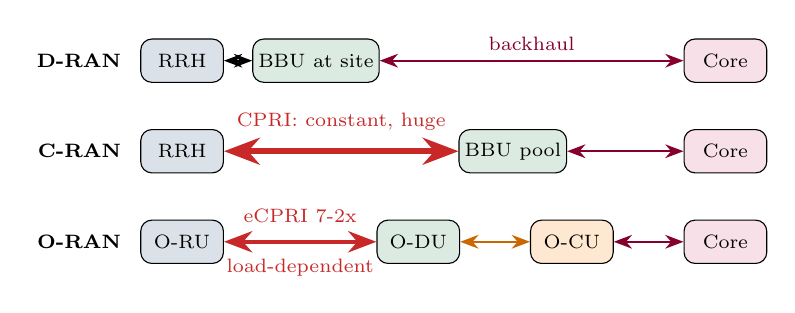
\begin{tikzpicture}[font=\scriptsize,>=Stealth,
  b/.style={draw,rounded corners,align=center,minimum height=0.55cm,minimum width=1.05cm,inner sep=2pt},
  row/.style={font=\scriptsize\bfseries,anchor=east}]
  \node[row] at (-0.25,0) {D-RAN};
  \node[b,fill=iitblue!15] (r1) at (0.4,0) {RRH};
  \node[b,fill=good!15] (b1) at (2.1,0) {BBU at site};
  \node[b,fill=purple!12] (c1) at (7.3,0) {Core};
  \draw[<->,thick] (r1) -- (b1);
  \draw[<->,thick,purple!70!black] (b1) -- node[above]{backhaul} (c1);
  \node[row] at (-0.25,-1.15) {C-RAN};
  \node[b,fill=iitblue!15] (r2) at (0.4,-1.15) {RRH};
  \node[b,fill=good!15] (b2) at (4.6,-1.15) {BBU pool};
  \node[b,fill=purple!12] (c2) at (7.3,-1.15) {Core};
  \draw[<->,line width=2.2pt,accent] (r2) -- node[above=3pt,text=accent]{CPRI: constant, huge} (b2);
  \draw[<->,thick,purple!70!black] (b2) -- (c2);
  \node[row] at (-0.25,-2.3) {O-RAN};
  \node[b,fill=iitblue!15] (r3) at (0.4,-2.3) {O-RU};
  \node[b,fill=good!15] (d3) at (3.4,-2.3) {O-DU};
  \node[b,fill=orange!18] (u3) at (5.35,-2.3) {O-CU};
  \node[b,fill=purple!12] (c3) at (7.3,-2.3) {Core};
  \draw[<->,line width=1.6pt,accent] (r3) -- node[above=3pt,text=accent]{eCPRI 7-2x} node[below=2pt,text=accent]{load-dependent} (d3);
  \draw[<->,thick,orange!80!black] (d3) -- (u3);
  \draw[<->,thick,purple!70!black] (u3) -- (c3);
\end{tikzpicture}
\end{column}
\begin{column}{0.42\textwidth}
\small
\begin{itemize}
  \item \textbf{C-RAN} pools baseband but CPRI ships samples at a \emph{constant} rate $\propto$ bandwidth $\times$ antennas, even for an idle cell.
  \item \textbf{O-RAN split 7-2x}: FFT stays in the O-RU; the fronthaul carries frequency-domain IQ \textbf{only for scheduled PRBs}, BFP-compressed, over Ethernet.
  \item Load now \textbf{follows the traffic} $\Rightarrow$ many cells can be \textbf{statistically multiplexed} on one link.
\end{itemize}
\end{column}
\end{columns}
\vspace{0.6em}
\begin{takeaway}
\faLightbulb[regular]\ \ Fronthaul load = number of \emph{scheduled PRB-layers} $\times$ bits per PRB-layer, not application bits. Both parts of the project rest on this fact.
\end{takeaway}
\end{frame}

% ---------------------------------------------------------------------
\begin{frame}{Why the fronthaul is the bottleneck}
\begin{columns}[c]
\begin{column}{0.47\textwidth}
\centering
\resizebox{\linewidth}{!}{%
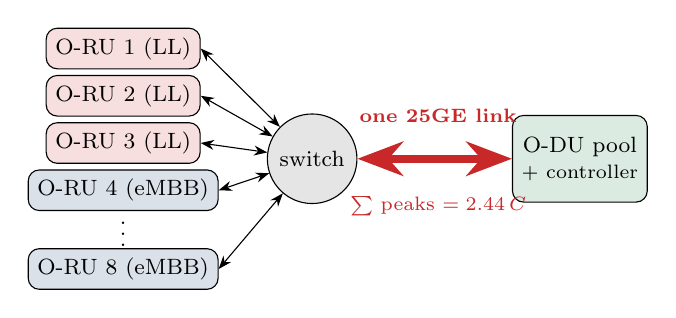
\begin{tikzpicture}[font=\footnotesize,>=Stealth,
   ru/.style={draw,fill=iitblue!15,rounded corners,minimum width=1.7cm,minimum height=0.5cm,align=center},
   ll/.style={draw,fill=accent!15,rounded corners,minimum width=1.7cm,minimum height=0.5cm,align=center}]
  \node[ll] (r1) at (0,2.4) {O-RU 1 (LL)};
  \node[ll] (r2) at (0,1.8) {O-RU 2 (LL)};
  \node[ll] (r3) at (0,1.2) {O-RU 3 (LL)};
  \node[ru] (r4) at (0,0.6) {O-RU 4 (eMBB)};
  \node at (0,0.15) {$\vdots$};
  \node[ru] (r8) at (0,-0.4) {O-RU 8 (eMBB)};
  \node[draw,fill=gray!20,circle,minimum size=0.95cm] (sw) at (2.4,1.0) {switch};
  \node[draw,fill=good!15,rounded corners,minimum height=1.1cm,align=center] (du) at (5.8,1.0) {O-DU pool\\\scriptsize + controller};
  \foreach \r in {r1,r2,r3,r4,r8} \draw[<->] (\r.east) -- (sw);
  \draw[<->,line width=3pt,accent] (sw) -- (du);
  \node[text=accent,font=\scriptsize\bfseries,align=center] at (4.0,1.55) {one 25GE link};
  \node[text=accent,font=\scriptsize,align=center] at (4.0,0.4) {$\sum$ peaks $= 2.44\,C$};
\end{tikzpicture}}\\[4pt]
\scriptsize 64-antenna cell: $\approx$34\,Gbit/s raw (16-bit IQ); 100\,MHz, 4 layers, BFP-9: $\approx$7.4\,Gbit/s peak
\end{column}
\begin{column}{0.51\textwidth}
\small
\begin{alertblock}{\faDatabase\ \ 1. Data are large, time is short}
BFP gives only $\approx$\textbf{2$\times$} over 16-bit IQ. Every 0.5\,ms slot the O-DU must invert a $K{\times}K$ Gram for all \textbf{273 PRBs}: numpy + LAPACK needs \textbf{3.2\,ms} for 16 users, i.e.\ \textbf{6$\times$ the slot}.
\end{alertblock}
\vspace{0.2em}
\begin{alertblock}{\faTrafficLight\ \ 2. The link is shared and smaller than the peak}
When bursts coincide someone loses data. LL cells tolerate only \textbf{2\,ms}. Budgets must be set every \textbf{10\,ms}, on 1\,ms-old telemetry, \emph{before} the traffic is seen.
\end{alertblock}
\end{column}
\end{columns}
\end{frame}

% ---------------------------------------------------------------------
\begin{frame}{Problem statement and our two levers}
\centering
\begin{tikzpicture}[font=\small,>=Stealth,
   lever/.style={draw,rounded corners=4pt,align=left,text width=6.5cm,inner sep=7pt,line width=0.8pt}]
  \node[lever,draw=iitblue,fill=iitblue!6] (A) at (0,0) {%
    \textbf{\textcolor{iitblue}{\faIcon{compress-arrows-alt}\ \ Part A: make the data smaller and the DU faster}}\\[4pt]
    \footnotesize Compress the per-slot IQ using its structure (low rank, delay sparsity) \emph{with error bounds}, and make the per-slot complex RZF precoder fit inside the \textbf{0.5\,ms} slot on a CPU.\\[4pt]
    \scriptsize CSEE \textbullet\ RAS-BFP \textbullet\ InverseNets \textbullet\ RMT-WS \textbullet\ fused C/AVX-512 kernel};
  \node[lever,draw=accent,fill=accent!5] (B) at (7.3,0) {%
    \textbf{\textcolor{accent}{\faNetworkWired\ \ Part B: share one link well}}\\[4pt]
    \footnotesize Every 10\,ms, before the traffic is known, set per-cell budgets on a shared 7-2x link so that the \textbf{priority-weighted fraction of bits that miss their deadline} is minimised.\\[4pt]
    \scriptsize $\rstar$ target \textbullet\ KKT newsvendor (B1) \textbullet\ Bayesian Transformer (B2) \textbullet\ BPN (B3)};
  \node[draw=good,line width=0.8pt,rounded corners=4pt,fill=good!8,text width=13.8cm,align=center,inner sep=6pt] (AB) at (3.65,-2.75) {%
    \textbf{A $\times$ B:} compression sets \emph{how much} load reaches the link;
    the allocation rule decides \emph{who} loses data when bursts coincide.};
  \draw[->,thick,iitblue] (A.south) -- (A.south |- AB.north);
  \draw[->,thick,accent] (B.south) -- (B.south |- AB.north);
\end{tikzpicture}
\end{frame}

% ---------------------------------------------------------------------
\begin{frame}{Headline results at a glance}
\begin{columns}[T]
\begin{column}{0.235\textwidth}
\kpi{iitblue}{\faCompress}{8.1$\times$}{channel IQ compression\\vs 16-bit at $-20$\,dB\\(O-RAN BFP: 2$\times$)}
\end{column}
\begin{column}{0.235\textwidth}
\kpi{iitblueL}{\faMicrochip}{14$\times$}{\texttt{libcmat} C/AVX-512 precoder\\0.226\,ms per slot\\(numpy + LAPACK: 3.21\,ms)}
\end{column}
\begin{column}{0.235\textwidth}
\kpi{gold!85!black}{\faBroadcastTower}{$-72\%$}{fronthaul with\\RU-side precoding,\\99.7\,\% of sum-rate}
\end{column}
\begin{column}{0.235\textwidth}
\kpi{good}{\faTrophy}{10/10}{scenarios of 3 families:\\BPN beats the strongest\\baselines by 3--25\,\%}
\end{column}
\end{columns}
\vspace{0.6em}
\small
\begin{columns}[T]
\begin{column}{0.48\textwidth}
\begin{itemize}
  \item \textbf{RMT-WS} inversion: \textbf{6 GEMMs} where Neumann-type schemes need $>$10; tracks users at \textbf{2.25 steps/slot} at walking speed.
\end{itemize}
\end{column}
\begin{column}{0.48\textwidth}
\begin{itemize}
  \item \textbf{KKT newsvendor rule}: best of 12 controllers in every scenario of 2 families; \textbf{$-11$ to $-43\,\%$} vs a point forecast, \textbf{20/20 seeds}.
\end{itemize}
\end{column}
\end{columns}
\end{frame}

% =====================================================================
\section{Part A: make the data smaller and the DU faster}
% =====================================================================

\begin{frame}{Part A system model: which IQ do we compress?}
\begin{columns}[T]
\begin{column}{0.5\textwidth}
\footnotesize
Per-slot frequency-domain matrix after OFDM demodulation:
\[ Y = H \odot X + W \in \mathbb{C}^{M\times N},\quad M{=}64,\ N{=}1200 \]
\begin{itemize}
  \item 3GPP TR 38.901 \textbf{TDL-A}, exponential antenna correlation.
  \item Raw rate, 16-bit I/Q: $\approx \mathbf{34.4}$\,Gbit/s per cell.
  \item Low rank and delay sparsity belong to $H$; random QAM data destroys them, so data IQ stays on BFP.
  \item \textbf{We compress channel-carrying IQ}: de-rotated reference symbols $Y \odot \bar X = H + \tilde W$ (DMRS/SRS) and channels shipped for RU-side precoding.
\end{itemize}
\end{column}
\begin{column}{0.48\textwidth}
\begin{block}{Two structures BFP ignores}
\begin{itemize}\small
  \item \textbf{Low rank}: correlated antennas $\Rightarrow$ rank $r \ll \min(M,N)$.
  \item \textbf{Delay sparsity}: few strong TDL taps $\Rightarrow$ energy in a few bins after IFFT across subcarriers.
\end{itemize}
\end{block}
\vspace{0.3em}
\centering
\resizebox{\linewidth}{!}{%
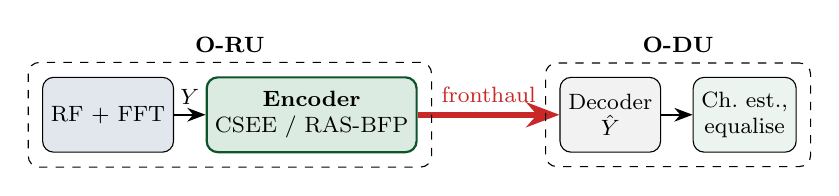
\begin{tikzpicture}[font=\footnotesize,>=Stealth,
   b/.style={draw,rounded corners,align=center,minimum height=0.95cm,inner sep=3pt},
   ours/.style={b,fill=good!15,draw=good!70!black,thick}]
  \node[b,fill=iitblue!12] (fft) {RF + FFT};
  \node[ours,right=0.4cm of fft] (enc) {\textbf{Encoder}\\CSEE / RAS-BFP};
  \node[b,fill=gray!10,right=1.8cm of enc] (dec) {Decoder\\$\hat Y$};
  \node[b,fill=good!8,right=0.4cm of dec] (eq) {Ch.\ est.,\\equalise};
  \draw[->,thick] (fft) -- node[above]{$Y$} (enc);
  \draw[->,line width=2pt,accent] (enc) -- node[above,text=accent]{fronthaul} (dec);
  \draw[->,thick] (dec) -- (eq);
  \node[draw,dashed,rounded corners,fit=(fft)(enc),inner sep=5pt,label={[font=\footnotesize\bfseries]above:O-RU}] {};
  \node[draw,dashed,rounded corners,fit=(dec)(eq),inner sep=5pt,label={[font=\footnotesize\bfseries]above:O-DU}] {};
\end{tikzpicture}}
\end{column}
\end{columns}
\vspace{0.2em}
\begin{takeaway}
\footnotesize Target NMSE $\approx -20$\,dB = noise floor at the 20\,dB operating SNR: compression error comparable to the estimation noise already present.
\end{takeaway}
\end{frame}

% ---------------------------------------------------------------------
\begin{frame}{Two structure-aware encoders with error bounds}
\begin{columns}[T]
\begin{column}{0.49\textwidth}
\begin{block}{CSEE: delay-domain sparse encoder}
\small
\begin{enumerate}
  \item $Y_d = \mathrm{IFFT}_N(Y)$ (row-wise)
  \item keep support $S = \mathrm{TopK}(|Y_d|)$
  \item per-antenna BFP on the $K$ kept taps
  \item O-DU: $\hat Y = \mathrm{FFT}_N(Y_d|_S)$
\end{enumerate}
\textbf{Theorem (error bound):}
\[ \mathrm{NMSE} \le \underbrace{\frac{\sigma^2_{\rm tail}}{\sigma^2_Y}}_{\text{truncation}} + \underbrace{\frac{\Delta^2}{12}\frac{K}{MN\sigma_Y^2}}_{\text{quantisation}} \]
Cost $O(MN\log N)$.
\end{block}
\end{column}
\begin{column}{0.49\textwidth}
\begin{block}{RAS-BFP: randomised sketch + QR}
\small
\begin{enumerate}
  \item SRHT sketch $Z = \Omega Y \in \mathbb{C}^{r\times N}$
  \item thin QR $Z^H = QR$, project $L = YQ$
  \item send $\mathrm{BFP}(L), \mathrm{BFP}(Q)$; $\ Y \approx LQ^H$
\end{enumerate}
\textbf{Theorem} (after Halko--Martinsson--Tropp), w.p.\ $\ge 1-\delta$:
\[ \|Y - LQ^H\|_F^2 \le (1+\varepsilon_r)\,\|Y - Y_r\|_F^2 \]
Rank under a bit budget: $r_{\max} = \big\lfloor B_{\rm total}/(2b(M+N))\big\rfloor$; pick $(r,b)$ on the budget line. Cost $O(rMN)$ vs $O(MN\min(M,N))$ for SVD.
\end{block}
\end{column}
\end{columns}
\end{frame}

% ---------------------------------------------------------------------
\begin{frame}{Compression results: 3--4$\times$ the ratio of the O-RAN standard}
\begin{columns}[c]
\begin{column}{0.44\textwidth}
\small
\centering
\begin{tabular}{lcc}
\toprule
Method & Ratio & Speed-up vs SVD \\
\midrule
O-RAN BFP ($b{=}8$) & 2.0$\times$ & n/a \\
Truncated SVD ($r{=}12$) & 8.1$\times$ & 1$\times$ \\
\ours \textbf{CSEE} ($K{=}300$) & \textbf{6.4$\times$} & \textbf{4--6$\times$} \\
\ours \textbf{RAS-BFP} ($r{=}12$) & \textbf{8.1$\times$} & \textbf{3--4$\times$} \\
\ours CSEE knee ($K{=}60$) & $\approx$\textbf{32$\times$} & n/a \\
\bottomrule
\end{tabular}\\[3pt]
{\scriptsize de-rotated reference-symbol IQ, NMSE $\approx -20$\,dB, $M{=}64$, $N{=}1200$, SNR 20\,dB; ratios vs 16-bit I/Q}
\vspace{0.5em}
\begin{itemize}\small
  \item RAS-BFP: the \textbf{same ratio as SVD}, encoded 3--4$\times$ faster.
  \item CSEE: 4--6$\times$ faster than SVD; $\approx$32$\times$ at $-19$\,dB at its Pareto knee.
  \item NMSE stable over SNR $-5$ to 30\,dB: no retuning as users move.
\end{itemize}
\end{column}
\begin{column}{0.55\textwidth}
\centering
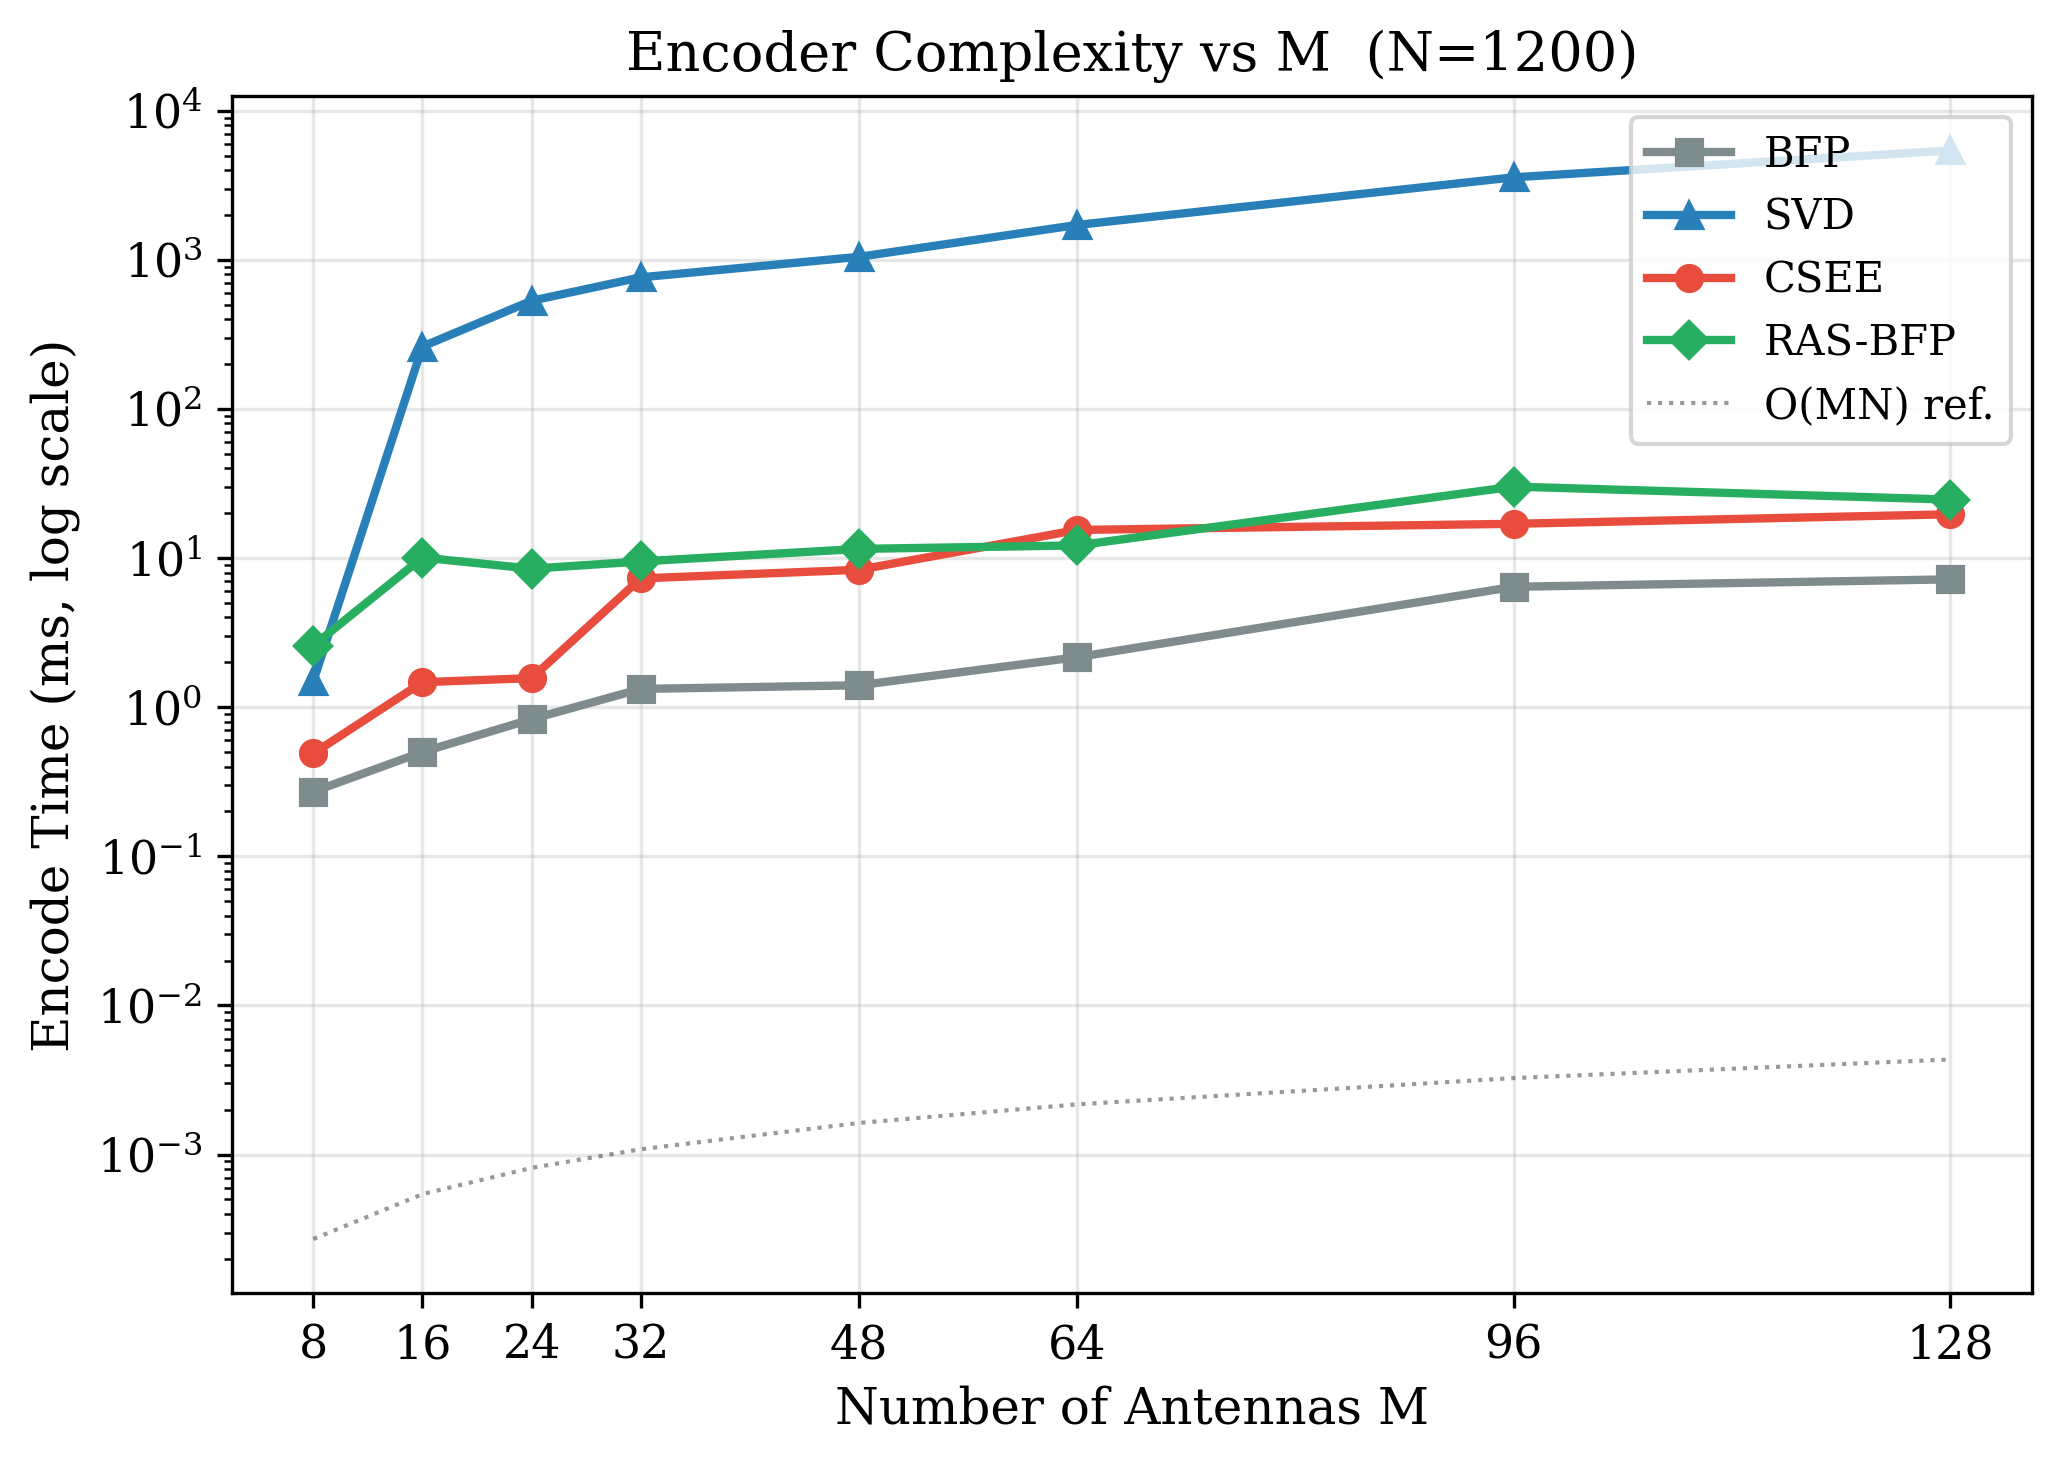
\includegraphics[width=0.95\linewidth]{exp2_complexity.png}\\[1pt]
{\scriptsize Encode time vs array size: truncated SVD grows fastest with $M$.}
\end{column}
\end{columns}
\end{frame}

% ---------------------------------------------------------------------
\begin{frame}{Inversion screening: learn the iteration, not the inverse}
\begin{columns}[c]
\begin{column}{0.42\textwidth}
\centering\small
\begin{tabular}{lcc}
\toprule
Method ($n{=}100$) & Mean & p95 \\
\midrule
\ours \textbf{InverseNet-Ultra} & \textbf{0.47} & \textbf{0.57} \\
LAPACK \texttt{getri} & 0.57 & 1.13 \\
\ours InverseNet-NS & 0.97 & 1.06 \\
Newton--Schulz & 1.27 & 1.71 \\
Gauss--Jordan & 1.97 & 3.40 \\
LU (scipy) & 3.36 & 6.09 \\
SVD & 10.2 & 20.8 \\
QR & 20.3 & 64.5 \\
\bottomrule
\end{tabular}\\[2pt]
{\scriptsize ms, CPU, one matrix per Python call, 200 held-out $A = G/\sqrt n + 2I$}
\end{column}
\begin{column}{0.56\textwidth}
\footnotesize
\textbf{Why:} MMSE equalisation, RZF precoding and our encoders need an inverse \emph{every slot}. Our learned inverters unroll Newton--Schulz and learn only its coefficients:
\[ X_{k+1} = X_k(\beta_k I - \gamma_k A X_k) \]
\begin{itemize}
  \item \textbf{InverseNet-NS}: 8 steps, learned $(\beta_k,\gamma_k)$ and initial scale.
  \item \textbf{InverseNet-Ultra}: a tiny hyper-network predicts $X_0$ from 4 matrix norms $\Rightarrow$ 2 steps fewer.
  \item Lowest mean latency, \textbf{2$\times$ lower p95} than LAPACK; fixed cost of batched GEMMs (GPU/NPU friendly).
\end{itemize}
\begin{takeaway}
\footnotesize Outcome: the \textbf{Newton--Schulz family with a good initial guess}, which RMT-WS develops for the real complex RZF workload.
\end{takeaway}
\end{column}
\end{columns}
\end{frame}

% ---------------------------------------------------------------------
\begin{frame}{RMT-WS: random-matrix-guided warm-start inversion}
\begin{columns}[c]
\begin{column}{0.47\textwidth}
\centering
\resizebox{\linewidth}{!}{%
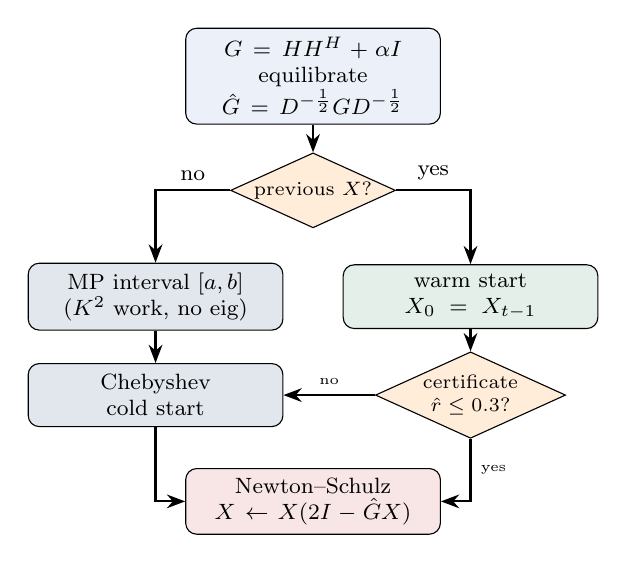
\begin{tikzpicture}[font=\footnotesize,>=Stealth,
   s/.style={draw,rounded corners,fill=soft,align=center,text width=3.0cm,minimum height=0.8cm},
   d/.style={draw,diamond,aspect=2.2,fill=orange!15,align=center,inner sep=0.5pt,font=\scriptsize},
   g/.style={s,fill=good!15}]
  \node[s] (g)    at (0,0)     {$G = HH^H + \alpha I$\\equilibrate $\hat G = D^{-\frac12} G D^{-\frac12}$};
  \node[d] (dec)  at (0,-1.45) {previous $X$?};
  \node[s,fill=iitblue!12] (int)  at (-2.0,-2.8) {MP interval $[a,b]$\\($K^2$ work, no eig)};
  \node[s,fill=iitblue!12] (cheb) at (-2.0,-4.05) {Chebyshev\\cold start};
  \node[s,fill=good!12] (warm) at (2.0,-2.8)  {warm start\\$X_0 = X_{t-1}$};
  \node[d] (cert) at (2.0,-4.05)  {certificate\\$\hat r \le 0.3$?};
  \node[g,fill=accent!12] (ns) at (0,-5.4) {Newton--Schulz\\$X \leftarrow X(2I - \hat G X)$};
  \draw[->,thick] (g) -- (dec);
  \draw[->,thick] (dec.west) -| node[pos=0.25,above]{no} (int.north);
  \draw[->,thick] (dec.east) -| node[pos=0.25,above]{yes} (warm.north);
  \draw[->,thick] (int) -- (cheb);
  \draw[->,thick] (warm) -- (cert);
  \draw[->,thick] (cert.west) -- node[above,font=\tiny]{no} (cheb.east);
  \draw[->,thick] (cheb.south) |- (ns.west);
  \draw[->,thick] (cert.south) |- node[pos=0.25,right,font=\tiny]{yes} (ns.east);
\end{tikzpicture}}
\end{column}
\begin{column}{0.51\textwidth}
\small
Real workload: per PRB and slot, $W = H^H(HH^H+\alpha I)^{-1}$, $\times 273$ PRBs in 0.5\,ms; 38.901 UMa near-far, TDL-A, angular spread, Rician, Jakes aging 3--120\,km/h.
\begin{enumerate}\footnotesize
  \item \textbf{Equilibrate}: removes the near-far power spread.
  \item \textbf{Moment-matched Marchenko--Pastur interval}: $v = \|\hat G\|_F^2/K - 1$, $[a,b] = 1 + v/\bar s \mp 2\sqrt v$; widens automatically for correlated/LoS channels.
  \item \textbf{Chebyshev} start, minimax-optimal on $[a,b]$; Newton--Schulz converges quadratically using GEMMs only.
  \item \textbf{Warm start} from the previous slot's inverse.
  \item \textbf{Residual certificate} (2 probes, $4K^2$ MACs) picks the number of steps or falls back to a cold start.
\end{enumerate}
\end{column}
\end{columns}
\end{frame}

% ---------------------------------------------------------------------
\begin{frame}{RMT-WS results: spectral interval and cold-start cost}
\begin{columns}[T]
\begin{column}{0.53\textwidth}
\textbf{Interval coverage} (lower / upper edge, 720 cases)\\[3pt]
\scriptsize
\begin{tabular}{lcc}
\toprule
Channel & Fixed-ratio MP + Weyl & \textbf{Moment-matched (ours)} \\
\midrule
i.i.d., equal gain & 98.9 / 99.3\,\% & \textbf{100 / 100\,\%} \\
UMa near-far & 99.6 / 99.9\,\% & \textbf{100 / 100\,\%} \\
12$^\circ$ spread + near-far & 96.8 / 99.4\,\% & \textbf{100 / 100\,\%} \\
3$^\circ$ spread + near-far & 61.1 / 94.7\,\% & \textbf{90.6 / 100\,\%} \\
Rician 6\,dB + 12$^\circ$ & 41.3 / 90.7\,\% & \textbf{84.0 / 100\,\%} \\
\bottomrule
\end{tabular}\\[6pt]
\centering
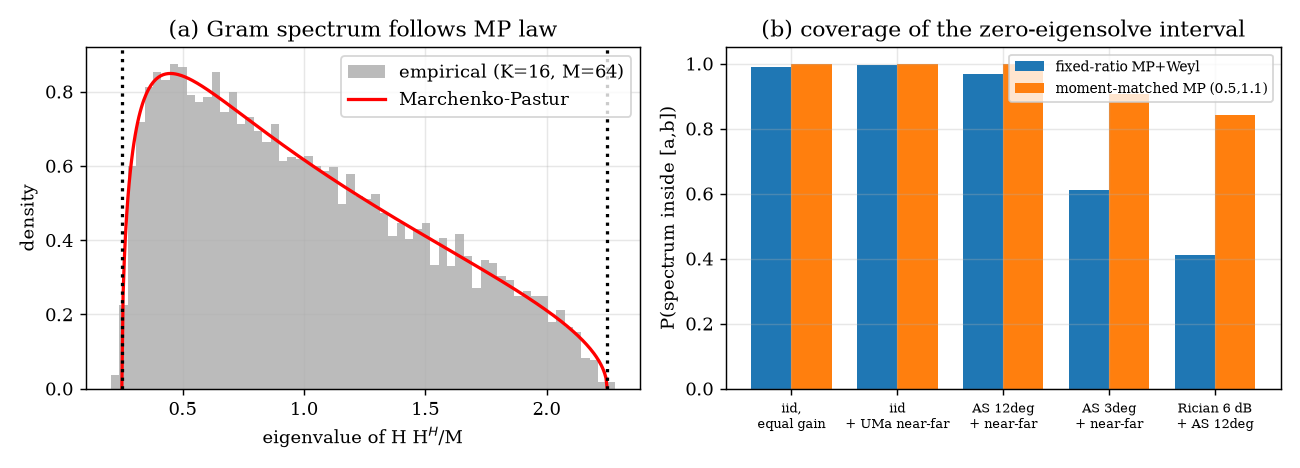
\includegraphics[width=0.98\linewidth]{exp5_spectrum_probability.png}
\end{column}
\begin{column}{0.45\textwidth}
\textbf{Complex GEMMs for $\le 1\,\%$ sum-rate loss}\\[3pt]
\small
\begin{tabular}{lcc}
\toprule
Method & 64/16 & 64/32 \\
\midrule
Neumann (Wu / Prabhu) & $>8$ & $>8$ \\
Newton--Neumann (Shao) & $>10$ & $>10$ \\
Newton--Schulz, classic & $>10$ & $>10$ \\
Block CG & 7 & 12 \\
Gauss--Seidel & 6 & $>12$ \\
\ours \textbf{Cheb-MP + NS (ours)} & \textbf{6} & \textbf{9} \\
\bottomrule
\end{tabular}\\[6pt]
\begin{itemize}\small
  \item Upper edge covered in \textbf{100\,\%} of cases on every channel type.
  \item \textbf{2$\times$} better lower-edge coverage on strongly correlated / LoS channels.
  \item Best of all methods at heavy load ($K/M = 0.5$).
\end{itemize}
\end{column}
\end{columns}
\end{frame}

% ---------------------------------------------------------------------
\begin{frame}{RMT-WS results: tracking at every user speed}
\begin{columns}[c]
\begin{column}{0.53\textwidth}
\small\textbf{Sum-rate loss / GEMMs per slot per PRB} ($K{=}16$, $M{=}64$)\\[3pt]
\footnotesize
\begin{tabular}{lccc}
\toprule
Speed & Warm GS $\times4$ & Warm CG $\times4$ & \textbf{RMT-WS} \\
\midrule
3\,km/h & 0.009\,\% / 4 & 0.013\,\% / 5 & \gd{0.006\,\% / 2.25} \\
30\,km/h & 0.63\,\% / 4 & 0.96\,\% / 5 & \gd{0.43\,\% / 5.2} \\
120\,km/h & 2.9\,\% / 4 & 5.5\,\% / 5 & \gd{0.12\,\% / 6.25} \\
\bottomrule
\end{tabular}
\vspace{0.4em}
\begin{itemize}\footnotesize
  \item Walking speed: \textbf{2.7$\times$ fewer GEMMs} than a cold start, 30$\times$ lower loss.
  \item 120\,km/h: fixed warm starts \hl{diverge}; the certificate falls back to a cold start: \textbf{24$\times$} lower loss than warm Gauss--Seidel.
  \item \textbf{Certificate audit}: 480 PRB cases, \textbf{0} accepted non-contractive steps.
  \item \textbf{Low precision} (8-bit mantissa): 0.15\,\% loss vs 0.88\,\% for direct Gauss--Jordan.
\end{itemize}
\end{column}
\begin{column}{0.45\textwidth}
\begin{block}{Doppler-to-warm-start law}
\[ r_0 \approx c\cdot 2\sqrt{\tfrac{K}{M-K}}\sqrt{1-\rho},\qquad 1-\rho \approx (\pi f_D T)^2 \]
\end{block}
\centering
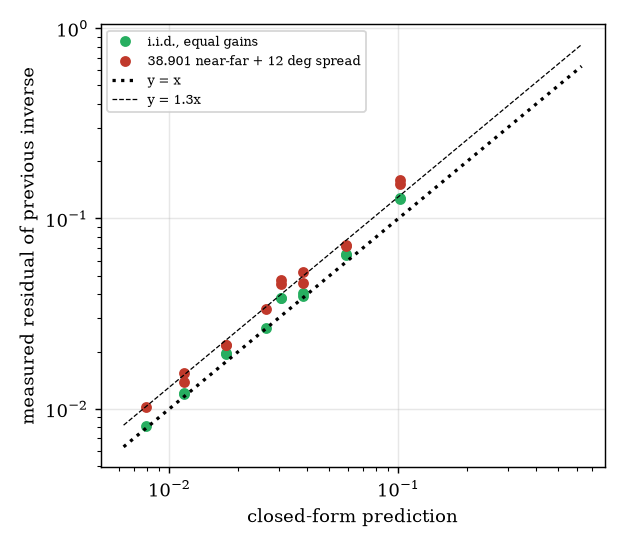
\includegraphics[height=3.15cm]{exp12_doppler_law.png}\\
{\scriptsize measured slope 1.00: warm start pays off up to \textbf{39\,km/h} ($K{=}16$), 60 ($K{=}8$), 23 ($K{=}32$)}
\end{column}
\end{columns}
\end{frame}

% ---------------------------------------------------------------------
\begin{frame}{Where should precoding run? $-72\,\%$ fronthaul at the RU}
\centering
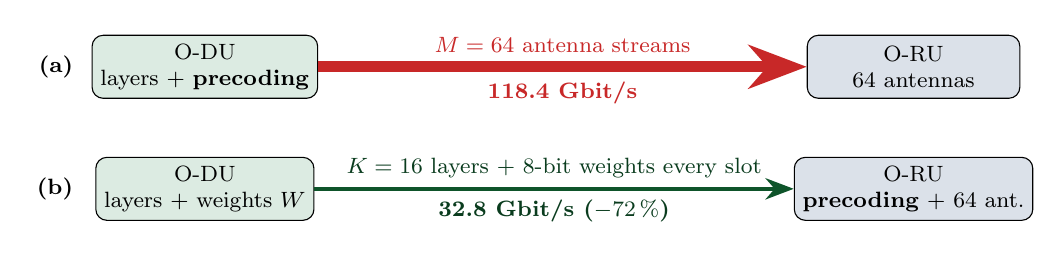
\begin{tikzpicture}[font=\footnotesize,>=Stealth,
   b/.style={draw,rounded corners,align=center,minimum height=0.8cm,inner sep=3pt,minimum width=2.7cm}]
  \node[b,fill=good!15] (du1) at (0,0) {O-DU\\layers + \textbf{precoding}};
  \node[b,fill=iitblue!15] (ru1) at (9.0,0) {O-RU\\64 antennas};
  \draw[->,line width=4pt,accent] (du1) -- node[above,text=accent]{$M = 64$ antenna streams} node[below,text=accent]{\textbf{118.4 Gbit/s}} (ru1);
  \node[anchor=east,font=\footnotesize\bfseries] at (-1.55,0) {(a)};
  \node[b,fill=good!15] (du2) at (0,-1.55) {O-DU\\layers + weights $W$};
  \node[b,fill=iitblue!15] (ru2) at (9.0,-1.55) {O-RU\\\textbf{precoding} + 64 ant.};
  \draw[->,line width=1.6pt,good!70!black] (du2) -- node[above,text=good!50!black]{$K = 16$ layers + 8-bit weights every slot} node[below,text=good!50!black]{\textbf{32.8 Gbit/s ($-72\,\%$)}} (ru2);
  \node[anchor=east,font=\footnotesize\bfseries] at (-1.55,-1.55) {(b)};
\end{tikzpicture}\\[6pt]
\small
\begin{tabular}{lcc}
\toprule
Architecture (100\,MHz, $M{=}64$, $K{=}16$, BFP-9) & Fronthaul & Sum-rate vs exact RZF \\
\midrule
DU precodes, sends 64 streams & 118.4 Gbit/s & 100\,\% \\
\ours \textbf{RU precodes, 16 layers + 8-bit weights} & \textbf{32.8 Gbit/s ($-72\,\%$)} & \textbf{99.7\,\%} \\
RU precodes, 16 layers + 6-bit weights & 32.0 Gbit/s ($-73\,\%$) & 96.7\,\% \\
\bottomrule
\end{tabular}
\vspace{0.4em}
\begin{takeaway}
At mobility the weights must be refreshed \textbf{every slot} (every 4 slots gives only 70\,\% of the rate at 30\,km/h): only viable with a fast per-slot precoder.
\end{takeaway}
\end{frame}

% ---------------------------------------------------------------------
\begin{frame}[fragile]{Kernel engineering: a fused RZF precoder in C/AVX-512/OpenMP}
\centering
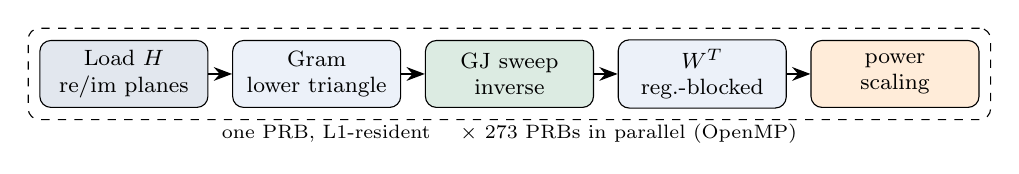
\begin{tikzpicture}[font=\footnotesize,>=Stealth,
   s/.style={draw,rounded corners,align=center,minimum height=0.85cm,text width=1.9cm,fill=soft},
   g/.style={s,fill=good!15}]
  \node[s,fill=iitblue!12] (h) {Load $H$\\re/im planes};
  \node[s,right=0.3cm of h] (gram) {Gram\\lower triangle};
  \node[g,right=0.3cm of gram] (inv) {GJ sweep\\inverse};
  \node[s,right=0.3cm of inv] (w) {$W^T$\\reg.-blocked};
  \node[s,right=0.3cm of w,fill=orange!15] (sc) {power\\scaling};
  \foreach \a/\b in {h/gram,gram/inv,inv/w,w/sc} \draw[->,thick] (\a) -- (\b);
  \node[draw,dashed,rounded corners,fit=(h)(gram)(inv)(w)(sc),inner sep=4pt,label={[font=\scriptsize,inner sep=1pt]below:one PRB, L1-resident \quad$\times$ 273 PRBs in parallel (OpenMP)}] {};
\end{tikzpicture}
\vspace{0.1em}
\begin{columns}[T]
\begin{column}{0.53\textwidth}
\begin{itemize}\footnotesize
  \item \textbf{One fused pass per PRB}: $H$ loaded once, no DRAM intermediates.
  \item \textbf{Split re/im planes} (SoA) so complex arithmetic vectorises.
  \item \textbf{Gauss--Jordan sweep}: $K$ rank-1 updates on contiguous rows; no pivoting since $G \succ 0$.
  \item \textbf{Profiling-driven} (\texttt{rdtsc}): weights 0.81$\to$\textbf{0.42\,ms}; inverse 6.4k$\to$\textbf{2.9k} cycles/PRB; AVX-512: 1.3--1.5$\times$ (1 thread), 2$\times$ (4 threads).
\end{itemize}
\end{column}
\begin{column}{0.45\textwidth}
\raggedright\textbf{\footnotesize Inner loop of the sweep inverse}
\begin{tcolorbox}[enhanced,colback=ink!4,colframe=ink!30,boxrule=0.4pt,arc=2pt,left=3pt,right=3pt,top=1pt,bottom=1pt]
\tiny
\begin{verbatim}
for (int i = 0; i < K; i++) {
  if (i == k) continue;
  float fr = ckr[i]*piv, fi = cki[i]*piv;
  float *ar = xr + i*K, *ai = xi + i*K;
  #pragma omp simd
  for (int j = 0; j < K; j++) {
    ar[j] -= fr*rkr[j] - fi*rki[j];
    ai[j] -= fr*rki[j] + fi*rkr[j];
  }
  ar[k] = -fr; ai[k] = -fi;
}
\end{verbatim}
\end{tcolorbox}
\begin{tcolorbox}[enhanced,colback=ink!4,colframe=ink!30,boxrule=0.4pt,arc=2pt,left=3pt,right=3pt,top=1pt,bottom=1pt]
\tiny
\begin{verbatim}
gcc -O3 -march=native -fopenmp -ffast-math \
    -mprefer-vector-width=512 -shared -fPIC
\end{verbatim}
\end{tcolorbox}
\footnotesize After tuning: weight formation 44--58\,\% of cycles at $\approx$30 flops/cycle ($\approx$ half AVX-512 peak).
\end{column}
\end{columns}
\end{frame}

% ---------------------------------------------------------------------
\begin{frame}{Kernel results: the whole precoder now fits the 0.5\,ms slot}
\begin{columns}[c]
\begin{column}{0.55\textwidth}
\centering
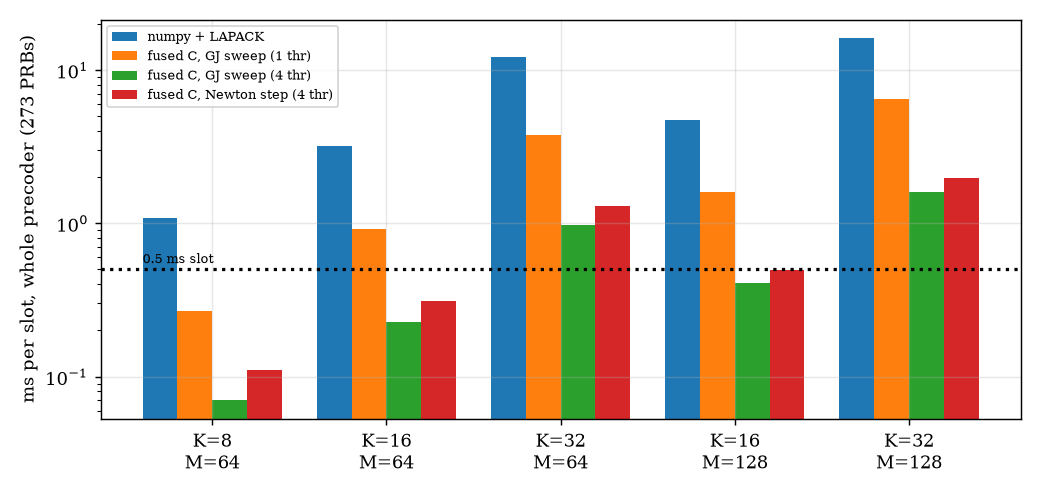
\includegraphics[width=\linewidth]{exp17_pipeline_kernel.png}\\
{\scriptsize whole precoder (Gram + inverse + weights), 273 PRBs, complex64, 4-core AVX-512 Xeon, median of 40 runs}
\end{column}
\begin{column}{0.43\textwidth}
\small
\setlength{\tabcolsep}{3.5pt}
\begin{tabular}{lccc}
\toprule
$K$, $M$ & numpy+LAPACK & \textbf{ours, 4 thr.} & gain \\
\midrule
8, 64 & 1.08\,ms & \gd{0.070} & 15$\times$ \\
\ours 16, 64 & 3.21\,ms & \gd{0.226} & \textbf{14$\times$} \\
32, 64 & 12.2\,ms & 0.97 & 12.5$\times$ \\
16, 128 & 4.71\,ms & \gd{0.41} & 11.6$\times$ \\
32, 128 & 16.3\,ms & 1.60 & 10$\times$ \\
\bottomrule
\end{tabular}
\vspace{0.4em}
\begin{itemize}\small
  \item $K \le 16$ fits the slot for the \emph{entire} precoder; none did before.
  \item Near-linear thread scaling: 0.92 $\to$ 0.45 $\to$ 0.23\,ms.
  \item Accuracy vs float64: sum-rate loss $\lesssim 10^{-6}\,\%$.
  \item Fused Newton step: fastest inverse (0.115\,ms vs 0.124 Cholesky, 1.6 LAPACK).
\end{itemize}
\end{column}
\end{columns}
\end{frame}

% ---------------------------------------------------------------------
\begin{frame}{\texttt{libcmat}: a batched complex linear-algebra library that beats LAPACK}
\begin{columns}[T]
\begin{column}{0.5\textwidth}
\footnotesize
\textbf{\small Why LAPACK is the wrong tool here}
\begin{itemize}
  \item LAPACK/numpy are tuned for \emph{one large} matrix; the O-DU needs \textbf{273 small} $K{\times}K$ problems every 0.5\,ms.
  \item Per-call overhead, separate Gram / inverse / product passes and DRAM round trips dominate at $K \le 32$.
\end{itemize}
\textbf{\small What \texttt{libcmat} does instead}
\begin{itemize}
  \item Batched API over all PRBs; one fused, L1-resident pass per PRB; split re/im planes for AVX-512 FMA; OpenMP across PRBs.
  \item Python binding via \texttt{ctypes}; complex64 accuracy checked against float64.
\end{itemize}
\vspace{0.2em}
\scriptsize
\setlength{\tabcolsep}{3pt}
\tiny
\begin{tabular}{>{\ttfamily}l l}
\toprule
\normalfont Routine & Computes (batched over PRBs) \\
\midrule
rzf\_fused\_chol & $G{=}HH^H{+}\alpha I$, $G^{-1}$, $W{=}H^H G^{-1}$, scaling \\
rzf\_fused\_ns & same, one warm Newton--Schulz step \\
ns\_step\_batch & $X \leftarrow X(2I{-}GX)$ + certificate \\
chol\_inverse\_batch & Hermitian pos.-definite inverse \\
rzf\_fused\_fp16 & weights in AVX512-FP16 complex FMA \\
\bottomrule
\end{tabular}
\end{column}
\begin{column}{0.48\textwidth}
\centering
\scriptsize
\setlength{\tabcolsep}{3pt}
\begin{tabular}{lccc}
\toprule
Inverse only, 273 PRBs & $K{=}8$ & $K{=}16$ & $K{=}32$ \\
\midrule
numpy + LAPACK & 0.354 & 1.594 & 7.883 \\
\ours \texttt{libcmat} Cholesky, 4 thr. & 0.042 & 0.124 & \textbf{0.572} \\
\ours \texttt{libcmat} NS step, 4 thr. & \textbf{0.036} & \textbf{0.115} & 0.645 \\
speed-up vs LAPACK & \gd{9.8$\times$} & \gd{13.9$\times$} & \gd{13.8$\times$} \\
\bottomrule
\end{tabular}\\[2pt]
{\tiny ms per slot, $M{=}64$, complex64, 4-core AVX-512 Xeon, median of 40 runs}\\[4pt]
\begin{tabular}{lcc}
\toprule
Whole precoder & 1 thread & 4 threads \\
\midrule
speed-up vs numpy + LAPACK & \gd{2.5--4.0$\times$} & \gd{10--15$\times$} \\
sum-rate loss vs float64 & \multicolumn{2}{c}{$\lesssim 10^{-6}\,\%$} \\
FP16 path, $K{=}32$, $M{=}128$ & \multicolumn{2}{c}{1.3$\times$ faster, $\le 0.5\,\%$ mean loss} \\
\bottomrule
\end{tabular}
\vspace{0.4em}
\begin{takeaway}
\scriptsize Faster than numpy + LAPACK at every tested size, even on a single core, at float64-level accuracy. We are preparing \texttt{libcmat} as a standalone open-source library and publication.
\end{takeaway}
\end{column}
\end{columns}
\end{frame}

% =====================================================================
\section{Part B: share one link well}
% =====================================================================

\begin{frame}{Part B setting: decide budgets before the traffic is seen}
\begin{columns}[T]
\begin{column}{0.52\textwidth}
\small
\begin{itemize}
  \item $N = 8$ cells on one 25GE link: \textbf{3 LL} ($D = 2$\,ms, weight 3), \textbf{5 eMBB} ($D = 10$\,ms, weight 1).
  \item 3\,\% reserved for C/M/S-plane $\Rightarrow C = 12.125$\,Mbit per 0.5\,ms slot; $\sum$ peaks $= 2.44\,C$.
  \item Every $T = 20$ slots (10\,ms) a coordinator sets budgets $r_i$, \textbf{held for the whole interval}, on telemetry $\tau = 1$\,ms old.
\end{itemize}
\begin{block}{Why decide in advance?}
\footnotesize near-RT RIC / E2 loops run at $\ge 10$\,ms; switch shaping is not reconfigured per slot; DU schedulers of different cells cannot consult each other inside the sub-ms pipeline.
\end{block}
\end{column}
\begin{column}{0.46\textwidth}
\centering
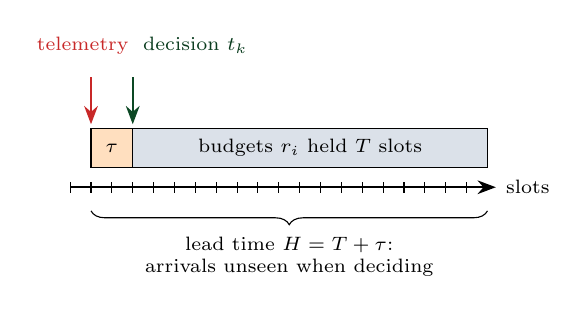
\begin{tikzpicture}[font=\scriptsize,>=Stealth,xscale=0.53]
  \draw[->,thick] (0,0) -- (10.2,0) node[right]{slots};
  \foreach \x in {0,0.5,...,9.5} \draw (\x,-0.07) -- (\x,0.07);
  \draw[fill=orange!25] (0.5,0.25) rectangle (1.5,0.75); \node at (1.0,0.5) {$\tau$};
  \draw[fill=iitblue!15] (1.5,0.25) rectangle (10.0,0.75); \node at (5.75,0.5) {budgets $r_i$ held $T$ slots};
  \draw[->,thick,accent] (0.5,1.4) -- (0.5,0.8); \node[text=accent,align=center] at (0.3,1.8) {telemetry};
  \draw[->,thick,good!60!black] (1.5,1.4) -- (1.5,0.8); \node[text=good!50!black,align=center] at (3.0,1.8) {decision $t_k$};
  \draw[decorate,decoration={brace,amplitude=5pt,mirror}] (0.5,-0.3) -- (10.0,-0.3) node[midway,below=6pt,align=center]{lead time $H = T + \tau$:\\arrivals unseen when deciding};
\end{tikzpicture}
\vspace{0.6em}
\begin{alertblock}{Question}
\small If each cell's need is available as a forecast \emph{distribution}, how should one shared link be split between cells with different deadlines and priorities?
\end{alertblock}
\end{column}
\end{columns}
\end{frame}

% ---------------------------------------------------------------------
\begin{frame}{System model and metric}
\begin{columns}[T]
\begin{column}{0.53\textwidth}
\small
\textbf{Cost of one PRB-layer per slot}, $b$-bit BFP:
\[ \beta(b) = (12\cdot 2\cdot b + 8)\cdot 14\cdot\kappa,\quad \beta(9) = 3387\text{ bits} \]
\pill{good}{A $\to$ B} \ \ \emph{Part A enters here}: compression sets $\beta$ and thus the load (BFP-6: $0.68\times$, BFP-12: $1.32\times$).\\[6pt]
\textbf{Fronthaul demand} (user bits $a_i$, spectral eff.\ $\eta_i$):
\[ d_i(t) = \lceil a_i(t)/\eta_i(t)\rceil\,\beta \]
Same user traffic can differ by 2--3$\times$ in fronthaul load.
\end{column}
\begin{column}{0.45\textwidth}
\small
\textbf{Decision} every $T$ slots:
\[ \textstyle\sum_i r_i \le C,\qquad 0 \le r_i \le \mathrm{cap}_i = 273\,L_i\,\beta \]
\begin{itemize}
  \item FIFO DU queue per cell; bits older than $D_i$ are \textbf{dropped} = deadline violations.
  \item Budgets enforce capacity, so the link never queues.
\end{itemize}
\end{column}
\end{columns}
\vspace{0.4em}
\begin{block}{Primary metric, fixed before any tuning}
\[ V_w = \frac{\sum_i w_i\,\mathrm{violated}_i}{\sum_i w_i\,\mathrm{arrived}_i}\qquad\text{(a dropped LL bit counts 3$\times$; lower is better)} \]
\end{block}
\end{frame}

% ---------------------------------------------------------------------
\begin{frame}{Part B in three steps: two initial experiments, one final design}
\centering
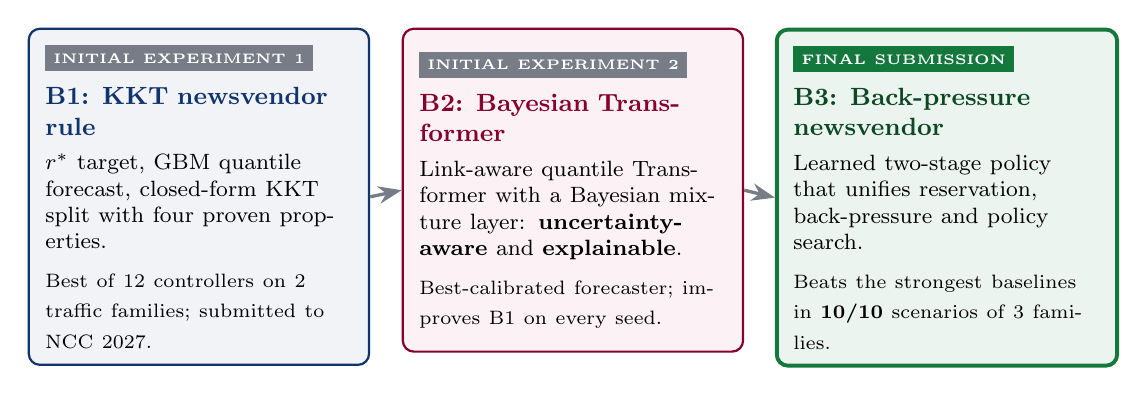
\begin{tikzpicture}[font=\small,>=Stealth,
   st/.style={draw,rounded corners=4pt,align=left,text width=3.9cm,minimum height=4.1cm,inner sep=6pt,line width=0.8pt,anchor=north}]
  \node[st,draw=iitblue,fill=iitblue!6] (b1) at (0,0) {%
    \colorbox{muted}{\tiny\bfseries\color{white}INITIAL EXPERIMENT 1}\\[4pt]
    \textbf{\textcolor{iitblue}{B1: KKT newsvendor rule}}\\[3pt]
    \footnotesize $\rstar$ target, GBM quantile forecast, closed-form KKT split with four proven properties.\\[3pt]
    \scriptsize Best of 12 controllers on 2 traffic families; submitted to NCC 2027.};
  \node[st,draw=purple!70!black,fill=purple!5] (b2) at (4.75,0) {%
    \colorbox{muted}{\tiny\bfseries\color{white}INITIAL EXPERIMENT 2}\\[4pt]
    \textbf{\textcolor{purple!70!black}{B2: Bayesian Transformer}}\\[3pt]
    \footnotesize Link-aware quantile Transformer with a Bayesian mixture layer: \textbf{uncertainty-aware} and \textbf{explainable}.\\[3pt]
    \scriptsize Best-calibrated forecaster; improves B1 on every seed.};
  \node[st,draw=good,fill=good!8,line width=1.4pt] (b3) at (9.5,0) {%
    \colorbox{good}{\tiny\bfseries\color{white}FINAL SUBMISSION}\\[4pt]
    \textbf{\textcolor{good!60!black}{B3: Back-pressure newsvendor}}\\[3pt]
    \footnotesize Learned two-stage policy that unifies reservation, back-pressure and policy search.\\[3pt]
    \scriptsize Beats the strongest baselines in \textbf{10/10} scenarios of 3 families.};
  \draw[->,very thick,muted] (b1.east) -- (b2.west);
  \draw[->,very thick,muted] (b2.east) -- (b3.west);
\end{tikzpicture}\\[8pt]
\begin{takeaway}
Between B2 and B3 we implemented all three solution families of the underlying POMDP (stochastic program, Lyapunov drift, policy search); B3 combines their strengths in one policy class.
\end{takeaway}
\end{frame}

% ---------------------------------------------------------------------
\begin{frame}{B1 \textbullet\ Key idea 1: forecast the deadline-feasible rate $\rstar$, not the volume}
\begin{columns}[c]
\begin{column}{0.55\textwidth}
\begin{tcolorbox}[enhanced,colback=soft,colframe=iitblue,boxrule=0.8pt,arc=3pt,halign=center]
Smallest constant rate at which \textbf{no bit misses its deadline}:
\[ \rstar(a, D) = \max_{1\le s\le e\le H} \frac{\sum_{t=s}^{e} a_t}{e - s + 1 + D} \]
\end{tcolorbox}
\small
\begin{itemize}
  \item Network-calculus service-curve condition; tight (verified to one PRB-layer in tests).
  \item Long deadline $\Rightarrow$ mean rate; short deadline $\Rightarrow$ peak burst rate.
  \item For 2\,ms cells: typically \textbf{2--3$\times$ the mean} and strongly \textbf{right-skewed}.
\end{itemize}
\end{column}
\begin{column}{0.43\textwidth}
\centering
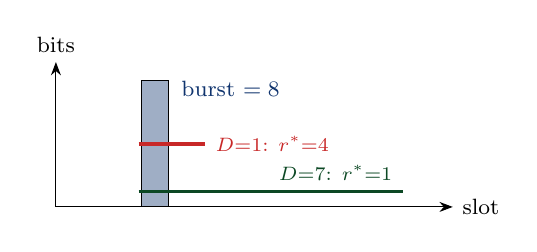
\begin{tikzpicture}[font=\footnotesize,>=Stealth,xscale=0.42,yscale=0.2]
  \draw[->] (0,0) -- (12,0) node[right]{slot};
  \draw[->] (0,0) -- (0,9.2) node[above]{bits};
  \foreach \x/\h in {3/8} \draw[fill=iitblue!40] (\x-0.4,0) rectangle (\x+0.4,\h);
  \node[iitblue,right] at (3.5,7.5) {burst $=8$};
  \draw[very thick,accent] (2.5,4) -- (4.5,4) node[right,font=\scriptsize]{$D{=}1$: $\rstar{=}4$};
  \draw[very thick,good!60!black] (2.5,1) -- (10.5,1) node[above left,font=\scriptsize]{$D{=}7$: $\rstar{=}1$};
\end{tikzpicture}\\[2pt]
\begin{block}{Every deadline-aware controller needs}
\[ \text{need}_i = \underbrace{B_i}_{\text{backlog / slack}} + \underbrace{\rstar_i}_{\text{future}} \]
\footnotesize Controllers differ only in how $\rstar_i$ is estimated and how a shortage is split.
\end{block}
\end{column}
\end{columns}
\vspace{0.2em}
\begin{takeaway}
A single predicted number is a poor basis for reserving a skewed quantity $\Rightarrow$ forecast a \textbf{range} (quantiles).
\end{takeaway}
\end{frame}

% ---------------------------------------------------------------------
\begin{frame}{B1 \textbullet\ Key idea 2: quantile forecast + closed-form KKT newsvendor split}
\begin{columns}[T]
\begin{column}{0.53\textwidth}
\small
\textbf{Forecaster:} gradient-boosted quantile regressors, $\alpha \in \{.05,.25,.5,.75,.9,.95\}$, 28 past-only features, 12\,s training; calibrated within $\approx$1 pp.\\[4pt]
\textbf{Surrogate:} expected weighted need served
\[ \max_{r}\ \textstyle\sum_i w_i\,\mathbb{E}\big[\min(B_i + \rstar_i,\ r_i)\big]\ \ \text{s.t.}\ \textstyle\sum_i r_i \le C \]
Separable and concave $\Rightarrow$ KKT gives the \textbf{global} optimum:
\begin{tcolorbox}[enhanced,colback=accent!5,colframe=accent,boxrule=0.8pt,arc=3pt,halign=center,top=0pt,bottom=0pt]
\[ r_i(\lambda) = \mathrm{clip}\Big(B_i + F_i^{-1}\big(1 - \lambda/w_i\big),\,0,\,\mathrm{cap}_i\Big) \]
\end{tcolorbox}
\footnotesize One price $\lambda$ for the whole link, 60-step bisection; $<0.1$\,ms for 8 cells.
\end{column}
\begin{column}{0.45\textwidth}
\centering
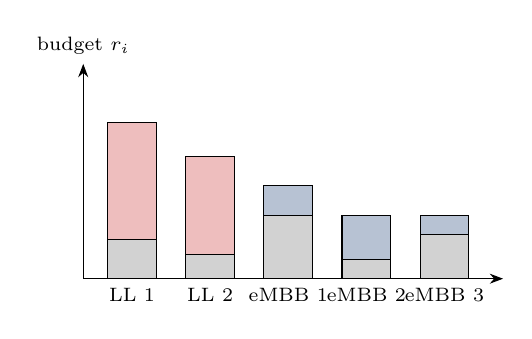
\begin{tikzpicture}[font=\scriptsize,>=Stealth,xscale=0.62,yscale=0.62]
  \draw[->] (0,0) -- (8.6,0);
  \draw[->] (0,0) -- (0,4.4) node[above]{budget $r_i$};
  \foreach \x/\b/\m/\lab/\col in {1/0.8/2.4/LL 1/accent,2.6/0.5/2.0/LL 2/accent,4.2/1.3/0.6/eMBB 1/iitblue,5.8/0.4/0.9/eMBB 2/iitblue,7.4/0.9/0.4/eMBB 3/iitblue}{
    \draw[fill=gray!35] (\x-0.5,0) rectangle (\x+0.5,\b);
    \draw[fill=\col!30] (\x-0.5,\b) rectangle (\x+0.5,\b+\m);
    \node[below] at (\x,0) {\lab};
  }
\end{tikzpicture}\\[2pt]
{\scriptsize\tikz\draw[fill=gray!35] (0,0) rectangle (0.25,0.15); backlog \quad
 \tikz\draw[fill=accent!30] (0,0) rectangle (0.25,0.15); LL $F^{-1}(0.8)$ \quad
 \tikz\draw[fill=iitblue!30] (0,0) rectangle (0.25,0.15); eMBB $F^{-1}(0.4)$}\\[2pt]
{\scriptsize toy example: $\lambda = 0.6$}
\vspace{0.3em}
\begin{exampleblock}{Intuition}
\footnotesize Every cell is cut at the \textbf{same priority-weighted risk}. Wide forecast or high priority $\Rightarrow$ more margin. Margins are \emph{derived}, not tuned.
\end{exampleblock}
\end{column}
\end{columns}
\end{frame}

% ---------------------------------------------------------------------
\begin{frame}{B1 \textbullet\ Four proven properties and the closed control loop}
\begin{columns}[T]
\begin{column}{0.47\textwidth}
\footnotesize
\begin{block}{P1 Feasibility}
For any forecast and $\lambda$: caps hold and $\sum_i r_i \le C$.
\end{block}
\begin{block}{P2 Equal weighted tail probability}
Interior optimum: $w_i(1 - F_i(r_i - B_i)) = \lambda$ for all cells.
\end{block}
\begin{block}{P3 Backlog first}
Any cell with $\lambda < w_i$ gets $\ge \min(B_i,\mathrm{cap}_i)$ before uncertain demand of an equal- or lower-weight cell.
\end{block}
\begin{block}{P4 Robustness to miscalibration}
$\sup|F_i - G_i| \le \epsilon \Rightarrow J_G(r^G) - J_G(r^F) \le 2\,\epsilon\, w_{\max}\, C$: loss grows at most \textbf{linearly} in $\epsilon$.
\end{block}
\end{column}
\begin{column}{0.51\textwidth}
\centering
\resizebox{\linewidth}{!}{%
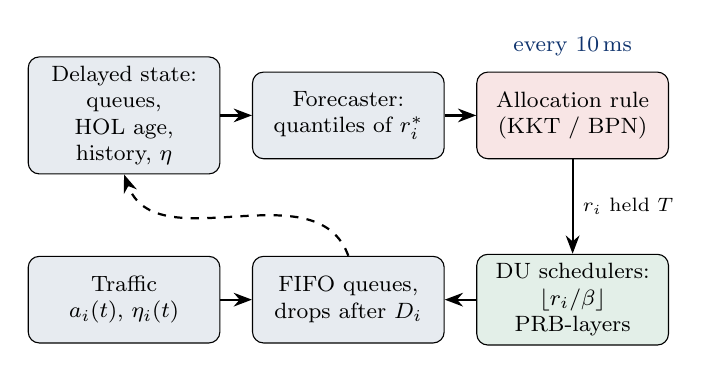
\begin{tikzpicture}[font=\footnotesize,>=Stealth,node distance=0.5cm and 0.4cm,
   st/.style={draw,rounded corners,fill=iitblue!10,align=center,minimum height=1.1cm,text width=2.2cm}]
  \node[st] (obs) {Delayed state:\\queues, HOL age,\\history, $\eta$};
  \node[st,right=of obs] (gbm) {Forecaster:\\quantiles of $\rstar_i$};
  \node[st,right=of gbm,fill=accent!12] (kkt) {Allocation rule\\(KKT / BPN)};
  \node[st,below=1.2cm of kkt,fill=good!12] (du) {DU schedulers:\\$\lfloor r_i/\beta\rfloor$ PRB-layers};
  \node[st,left=of du] (q) {FIFO queues,\\drops after $D_i$};
  \node[st,left=of q] (traffic) {Traffic\\$a_i(t)$, $\eta_i(t)$};
  \draw[->,thick] (obs) -- (gbm);
  \draw[->,thick] (gbm) -- (kkt);
  \draw[->,thick] (kkt) -- node[right,font=\scriptsize]{$r_i$ held $T$} (du);
  \draw[->,thick] (du) -- (q);
  \draw[->,thick] (traffic) -- (q);
  \draw[->,thick,dashed] (q.north) to[out=110,in=-70] (obs.south);
  \node[above=0.08cm of kkt,text=iitblue] {every 10\,ms};
\end{tikzpicture}}
\vspace{0.4em}
\begin{itemize}\footnotesize
  \item Edge cases handled: non-finite forecast $\to$ window quantiles; zero demand $\to$ zero budget + headroom; link not binding $\to$ full predictive support.
  \item The forecaster and the allocation rule are the two blocks we improve in B2 and B3.
\end{itemize}
\end{column}
\end{columns}
\end{frame}

% ---------------------------------------------------------------------
\begin{frame}{A fair evaluation by construction}
\begin{columns}[T]
\begin{column}{0.33\textwidth}
\begin{tcolorbox}[enhanced,colback=iitblue!5,colframe=iitblue,boxrule=0.6pt,arc=3pt,title={\faRandom\ \ Family S: synthetic, bursty},fonttitle=\footnotesize\bfseries,colbacktitle=iitblue,height=2.9cm]
\scriptsize Gamma background + ON/OFF bursts with \textbf{Pareto sojourns}, slow regimes, SE drift.\\[3pt]
low 0.50, moderate 0.65, high 0.80, flash crowds, \textbf{held-out shift}.
\end{tcolorbox}
\end{column}
\begin{column}{0.33\textwidth}
\begin{tcolorbox}[enhanced,colback=good!5,colframe=good,boxrule=0.6pt,arc=3pt,title={\faBroadcastTower\ \ Family G: 3GPP},fonttitle=\footnotesize\bfseries,colbacktitle=good,height=2.9cm]
\scriptsize TR 38.901 UMa, 7 sites, Jakes fading, TS 38.214 CQI; FTP Model 3 (eMBB), XR video 60\,fps (LL); demand = PRB-scheduler output. \textbf{Nothing hand-designed.}
\end{tcolorbox}
\end{column}
\begin{column}{0.33\textwidth}
\begin{tcolorbox}[enhanced,colback=accent!5,colframe=accent,boxrule=0.6pt,arc=3pt,title={\faProjectDiagram\ \ Family M: Markov},fonttitle=\footnotesize\bfseries,colbacktitle=accent,height=2.9cm]
\scriptsize Markov-modulated Gamma sources (idle / normal / burst); moderate, high and a \textbf{semi-Markov held-out shift}.
\end{tcolorbox}
\end{column}
\end{columns}
\vspace{0.9em}
\begin{columns}[T]
\begin{column}{0.5\textwidth}
\footnotesize
\textbf{12 reference controllers in B1}, 19+ in the extended study: static, reactive proportional, MaxWeight, deadline-aware reactive, \textbf{point forecast} (same model, one number), fixed global quantile, window quantiles (no ML), oracles (reference only).
\end{column}
\begin{column}{0.48\textwidth}
\footnotesize
\begin{itemize}
  \item 20 test seeds $\times$ 20{,}000 slots; \textbf{identical traces} and stale observations for all.
  \item Disjoint train / val / test seeds; forecasters frozen before test.
  \item \textbf{Paired} bootstrap 95\,\% CI + Holm-corrected Wilcoxon.
\end{itemize}
\end{column}
\end{columns}
\end{frame}

% ---------------------------------------------------------------------
\begin{frame}{B1 \textbullet\ Main result: best implementable controller everywhere}
\centering
\scriptsize
\setlength{\tabcolsep}{4pt}
\begin{tabular}{lccccc}
\toprule
$V_w$ [\%], Family S, 20 seeds & low 0.50 & moderate 0.65 & high 0.80 & flash crowds & shift (held-out) \\
\midrule
Static equal share & 4.45 & 9.65 & 15.46 & 19.15 & 22.31 \\
Reactive proportional & 0.83 & 4.11 & 9.20 & 12.27 & 11.70 \\
MaxWeight & 0.90 & 4.85 & 11.54 & 15.24 & 12.31 \\
Deadline-aware reactive & 0.52 & 4.24 & 11.03 & 14.51 & 12.56 \\
Point forecast (GBM median) & 0.27 & 3.23 & 9.70 & 13.33 & 11.30 \\
Fixed global quantile (0.75) & 0.34 & 4.35 & 11.76 & 15.09 & 12.85 \\
Proposed, window quantiles (no ML) & 0.25 & 2.57 & 8.72 & 12.67 & 10.22 \\
\ours \textbf{Proposed (GBM + KKT)} & \textbf{0.15} & \textbf{2.15} & \textbf{8.00} & \textbf{11.76} & \textbf{10.04} \\
\midrule
\gray{Oracle water-fill (reference)} & \gray{0.07} & \gray{1.62} & \gray{6.89} & \gray{10.16} & \gray{6.69} \\
\bottomrule
\end{tabular}
\vspace{0.6em}
\begin{columns}[T]
\begin{column}{0.56\textwidth}
\begin{exampleblock}{Paired per seed: 20/20 seeds, every scenario, $p<0.01$}
\footnotesize\setlength{\tabcolsep}{3pt}
\begin{tabular}{@{}ll@{\hspace{8pt}}ll@{}}
vs point forecast & \gd{$-11$ to $-43\,\%$} & vs fixed quantile & \gd{$-22$ to $-54\,\%$}\\
vs deadline-aware & \gd{$-19$ to $-70\,\%$} & vs MaxWeight & \gd{$-18$ to $-83\,\%$}
\end{tabular}
\end{exampleblock}
\end{column}
\begin{column}{0.42\textwidth}
\begin{alertblock}{Weakest case}
\footnotesize Only $-4\,\%$ vs reactive proportional under flash crowds (16/20 seeds): it starves LL cells but serves eMBB better.
\end{alertblock}
\end{column}
\end{columns}
\end{frame}

% ---------------------------------------------------------------------
\begin{frame}{B1 \textbullet\ Where the gain comes from}
\begin{columns}[c]
\begin{column}{0.52\textwidth}
\centering
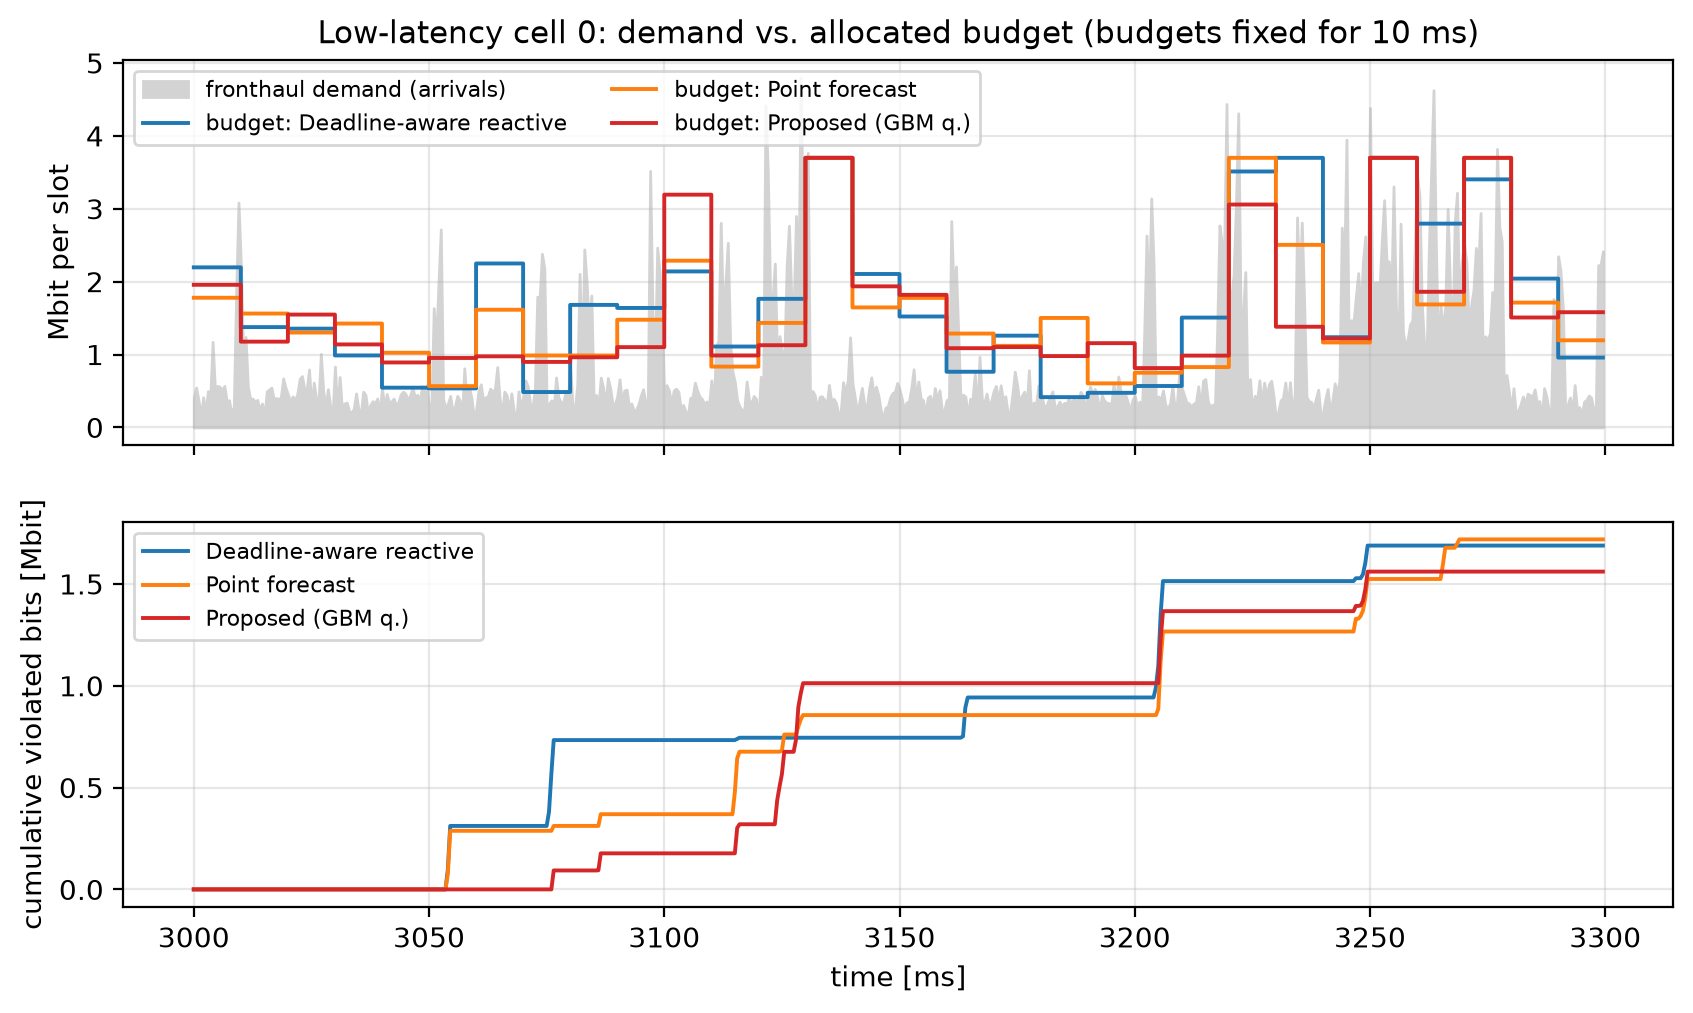
\includegraphics[width=\linewidth]{fig6_demo_timeseries.png}\\
{\scriptsize One LL cell: grey = demand, steps = budgets held 10\,ms. The reactive controller is \textbf{one interval late} at every burst; the KKT rule raises the budget at burst onset, where the forecast range is wide.}
\end{column}
\begin{column}{0.46\textwidth}
\small
\textbf{Deadline-aware controllers, S high}\\[3pt]
\begin{tabular}{lccc}
\toprule
Method & eMBB viol. & Util. & Jain \\
\midrule
Deadline-aware & 16.5\,\% & 69.3\,\% & 0.995 \\
Point forecast & 16.0\,\% & 70.1\,\% & 0.994 \\
Fixed quantile & 22.0\,\% & 67.0\,\% & 0.985 \\
\ours \textbf{Proposed} & \textbf{12.3\,\%} & \textbf{72.2\,\%} & \textbf{0.997} \\
\bottomrule
\end{tabular}
\vspace{0.5em}
\begin{itemize}\footnotesize
  \item Margin only where the forecast is wide $\Rightarrow$ lowest eMBB loss, highest utilisation, best fairness.
  \item One global quantile over-protects LL and wastes a third of its allocation.
\end{itemize}
\end{column}
\end{columns}
\end{frame}

% ---------------------------------------------------------------------
\begin{frame}{B1 \textbullet\ Ablations and standards-based 3GPP traffic}
\begin{columns}[T]
\begin{column}{0.48\textwidth}
\textbf{What carries the gain?} (all else fixed)\\[4pt]
\small
\begin{enumerate}
  \item \textbf{Range vs single number} (same model): $-11$ to $-43\,\%$, 20/20 seeds everywhere $\Rightarrow$ \emph{representing uncertainty matters}.
  \item \textbf{Per-cell KKT level vs one global level}: $-22$ to $-54\,\%$ $\Rightarrow$ the level must be set \emph{per cell by the link}.
  \item \textbf{GBM vs window (no-ML) quantiles}: GBM adds $-7$ to $-37\,\%$; even the no-ML version beats the point forecast everywhere.
\end{enumerate}
\begin{takeaway}
The rule ($\rstar$ target + KKT split) carries the method; the learned forecaster adds on top.
\end{takeaway}
\end{column}
\begin{column}{0.5\textwidth}
\textbf{Family G (3GPP)}, $V_w$ [\%]\\[3pt]
\scriptsize
\begin{tabular}{lccc}
\toprule
Method & mod.\ 0.65 & high 0.80 & unweighted \\
\midrule
Reactive prop. & 12.05 & 15.94 & 15.0 \\
MaxWeight & 17.51 & 25.79 & 19.7 \\
Deadline-aware & 8.95 & 11.53 & 18.5 \\
Point forecast & 6.00 & 8.98 & 16.6 \\
Window quantiles & 6.18 & 9.01 & 16.0 \\
\ours \textbf{Proposed} & \textbf{5.08} & \textbf{8.01} & \textbf{14.4} \\
Transfer (trained on S) & 6.99 & 9.89 & 14.3 \\
\midrule
\gray{Oracle + KKT} & \gray{3.47} & \gray{6.06} & \gray{11.1} \\
\bottomrule
\end{tabular}
\vspace{0.3em}
\begin{itemize}\footnotesize
  \item Reproduces on traffic we did not design: best at both loads, 20/20 seeds.
  \item High load: $-11\,\%$ vs point, $-31\,\%$ vs deadline-aware, $-50\,\%$ vs reactive.
\end{itemize}
\end{column}
\end{columns}
\end{frame}

% ---------------------------------------------------------------------
\begin{frame}{B1 \textbullet\ Robustness, operating range and the A $\times$ B experiment}
\begin{columns}[T]
\begin{column}{0.33\textwidth}
\textbf{\small Miscalibration} (P4 in practice)\\[2pt]
\centering
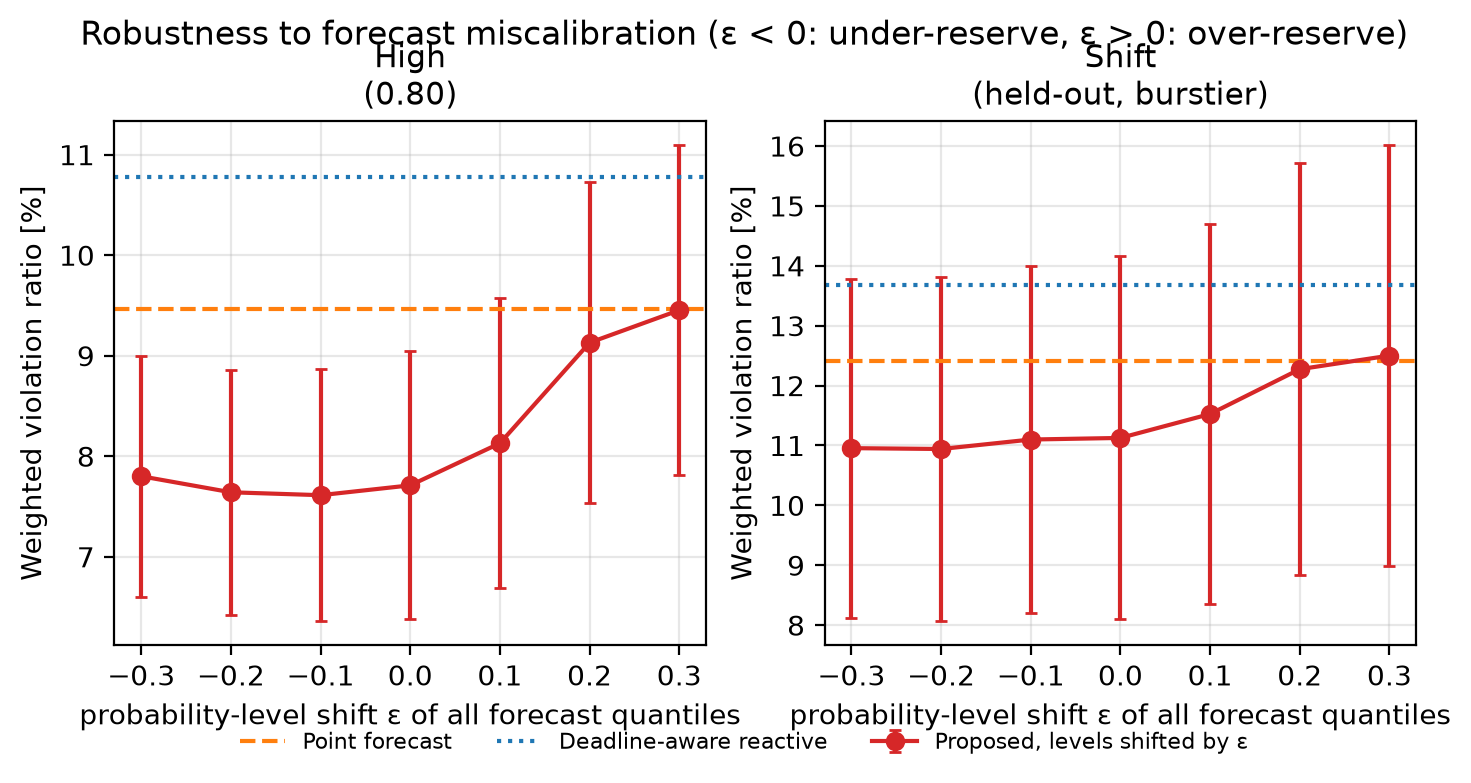
\includegraphics[width=\linewidth]{fig10_miscalibration.png}\\
\raggedright\scriptsize Every quantile level shifted by $\epsilon$: under-reserving is absorbed by $\lambda$; at $\epsilon{=}{+}0.3$ the rule (9.45\,\%) still matches the point forecast (9.46\,\%).
\end{column}
\begin{column}{0.31\textwidth}
\textbf{\small Interval $T$ and delay $\tau$} (S high)\\[2pt]
\scriptsize
\setlength{\tabcolsep}{3pt}
\begin{tabular}{lccc}
\toprule
$T$ & React. & Point & \textbf{Prop.} \\
\midrule
2\,ms & 3.91 & 6.57 & \gd{3.07} \\
5\,ms & 7.42 & 7.53 & \gd{5.07} \\
10\,ms & 8.91 & 9.46 & \gd{7.71} \\
\midrule
$\tau$ & \multicolumn{3}{c}{Prop.\ vs reactive} \\
\midrule
0\,ms & \multicolumn{3}{c}{6.85 ($-16\,\%$)} \\
1\,ms & \multicolumn{3}{c}{7.71 ($-13\,\%$)} \\
2.5\,ms & \multicolumn{3}{c}{8.77 ($-11\,\%$)} \\
5\,ms & \multicolumn{3}{c}{11.07 ($-2\,\%$)} \\
\bottomrule
\end{tabular}\\[2pt]
At $T{=}2$\,ms it beats even the oracle water-fill.
\end{column}
\begin{column}{0.33\textwidth}
\textbf{\small Part A $\times$ Part B}\\[2pt]
\scriptsize same user traffic, only BFP width changes $\beta$\\[3pt]
\setlength{\tabcolsep}{3pt}
\begin{tabular}{lcccc}
\toprule
BFP & load & React. & Point & \textbf{Prop.} \\
\midrule
6 bit & 0.44 & 0.22 & 0.15 & \gd{0.11} \\
9 bit & 0.65 & 3.90 & 3.00 & \gd{1.96} \\
\bottomrule
\end{tabular}
\vspace{0.4em}
\begin{tcolorbox}[enhanced,colback=good!8,colframe=good,boxrule=0.5pt,arc=2pt,left=3pt,right=3pt]
\scriptsize \textbf{Compression sets the regime; allocation decides the loss inside it.} At 0.65 load the rule \textbf{halves} reactive control's loss. Near full load no split helps: Part A must bring the load down.
\end{tcolorbox}
\end{column}
\end{columns}
\end{frame}

% ---------------------------------------------------------------------
\begin{frame}{B2 \textbullet\ LCQT: a Bayesian, link-aware quantile Transformer}
\centering
\resizebox{\linewidth}{!}{%
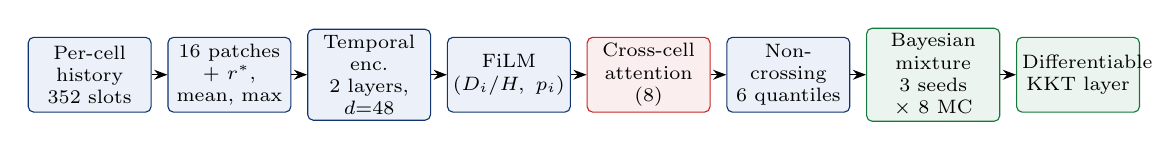
\begin{tikzpicture}[font=\scriptsize,>=Stealth,
    box/.style={draw=iitblue,fill=soft,rounded corners=2pt,align=center,minimum height=0.95cm,text width=1.42cm,inner sep=2pt},
    hot/.style={box,draw=accent,fill=accent!8},
    grn/.style={box,draw=good,fill=good!8}]
  \node[box] (hist) {Per-cell history\\352 slots};
  \node[box,right=0.2cm of hist] (patch) {16 patches\\+ $\rstar$, mean, max};
  \node[box,right=0.2cm of patch] (enc) {Temporal enc.\\2 layers, $d{=}48$};
  \node[box,right=0.2cm of enc] (film) {FiLM\\$(D_i/H,\ p_i)$};
  \node[hot,right=0.2cm of film] (cross) {Cross-cell\\attention (8)};
  \node[box,right=0.2cm of cross] (head) {Non-crossing\\6 quantiles};
  \node[grn,right=0.2cm of head,text width=1.55cm] (bayes) {Bayesian mixture\\3 seeds $\times$ 8 MC};
  \node[grn,right=0.2cm of bayes,text width=1.42cm] (kkt) {Differentiable\\KKT layer};
  \foreach \a/\b in {hist/patch,patch/enc,enc/film,film/cross,cross/head,head/bayes,bayes/kkt} \draw[->] (\a) -- (\b);
\end{tikzpicture}}\\[6pt]
\begin{columns}[T]
\begin{column}{0.47\textwidth}
\footnotesize
\begin{itemize}
  \item Built on PatchTST, iTransformer, TFT, FiLM, deep ensembles and MC dropout, plus \textbf{six shared-link modifications}.
  \item \textbf{Mixture} $\hat F_i = \frac{1}{MS}\sum_s F_i^{(s)}$ instead of averaged quantiles: uncertain cells get wider margins.
  \item KKT layer: implicit gradient $\partial\lambda^\ast/\partial q$ through the binding link; matches numpy allocator to $10^{-6}$.
  \item 63k parameters, $\approx$6\,min CPU training.
\end{itemize}
\end{column}
\begin{column}{0.51\textwidth}
\footnotesize
\setlength{\tabcolsep}{3.5pt}
\begin{tabular}{lccc}
\toprule
Forecast quality & Pinball & \makecell{90\,\% cov.\\(shift)} & \makecell{LL $q_{95}$ cov.\\(shift)} \\
\midrule
GBM (B1) & 0.0224 & n/a & n/a \\
LCQT & 0.0214 & 0.795 & 0.855 \\
\ours \textbf{Bayesian (3 $\times$ 8)} & \textbf{0.0213} & \textbf{0.808} & \textbf{0.873} \\
\bottomrule
\end{tabular}\\[5pt]
\begin{itemize}
  \item Pinball loss $-4.5\,\%$ and a 90\,\% interval 8\,\% narrower, at \emph{higher} coverage than GBM.
  \item Best calibration of all models under the held-out shift.
  \item Closed loop with the B1 KKT rule: \gd{improves on GBM on 20/20 test seeds} at low, moderate and high load.
  \item With the final B3 policy it gives the \textbf{best results of the project}.
\end{itemize}
\end{column}
\end{columns}
\end{frame}

% ---------------------------------------------------------------------
\begin{frame}{B2 \textbullet\ Uncertainty-aware and explainable by design}
\centering
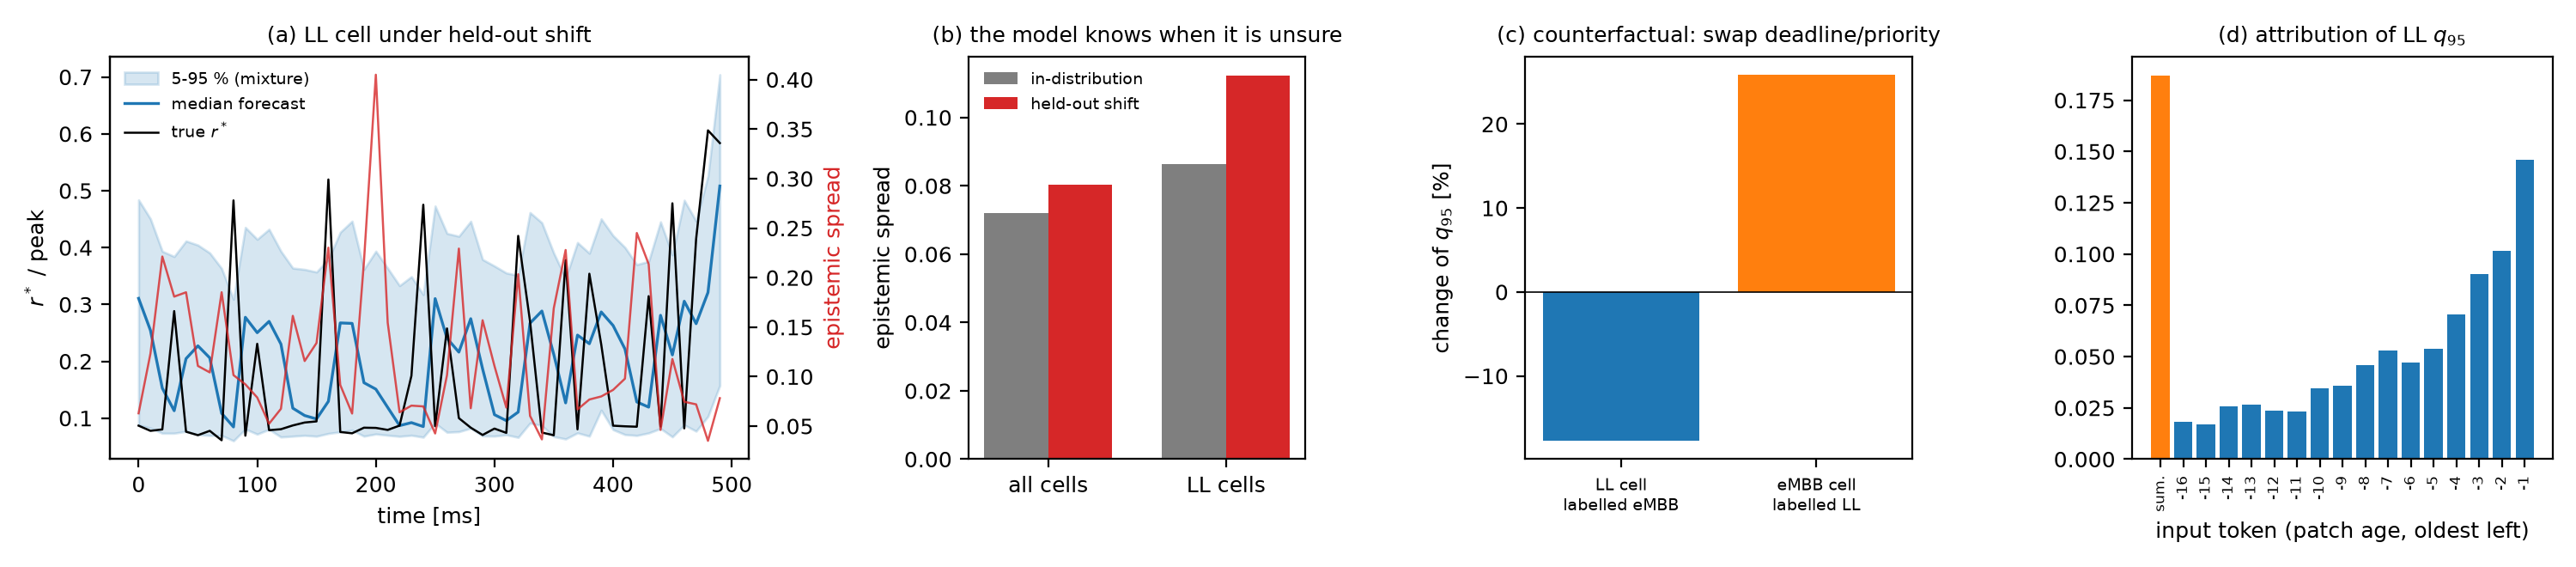
\includegraphics[height=2.75cm]{fig_bayes_explain.png}\\[-2pt]
{\tiny (a) LL cell under held-out shift, epistemic spread in red \textbullet\ (b) posterior disagreement \textbullet\ (c) FiLM counterfactual \textbullet\ (d) gradient $\times$ input attribution of LL $q_{95}$}\\[2pt]
\begin{columns}[T]
\begin{column}{0.49\textwidth}
\begin{block}{\faIcon{question-circle}\ \ Uncertainty-aware}
\footnotesize
\begin{itemize}
  \item 24 posterior samples (3 seeds $\times$ 8 MC dropout) separate \textbf{epistemic} (model) from \textbf{aleatoric} (traffic) uncertainty.
  \item Held-out shift: epistemic spread of LL forecasts \textbf{+30\,\%} (0.086 $\to$ 0.112); the model \emph{knows} when traffic is unfamiliar.
  \item The mixture widens those intervals, so the link reserves more where it is less sure.
\end{itemize}
\end{block}
\end{column}
\begin{column}{0.49\textwidth}
\begin{block}{\faIcon{search}\ \ Explainable}
\footnotesize
\begin{itemize}
  \item \textbf{Counterfactual}: LL cell relabelled eMBB $\Rightarrow$ $q_{95}$ \textbf{$-18\,\%$}; eMBB relabelled LL $\Rightarrow$ \textbf{+26\,\%}: it reserves for deadline and priority.
  \item \textbf{Attribution}: newest 4 of 16 history patches carry \textbf{41\,\%} of the LL $q_{95}$; summary features 19\,\%.
  \item Every budget reads as backlog + quantile at risk $1 - \lambda/w_i$.
\end{itemize}
\end{block}
\end{column}
\end{columns}
\end{frame}

% ---------------------------------------------------------------------
\begin{frame}{Towards B3 \textbullet\ We implemented all three POMDP solution families}
\begin{columns}[T]
\begin{column}{0.45\textwidth}
\footnotesize
\textbf{POMDP}: state = queue age profiles, hidden traffic state, SE; action held $T$ slots $\Rightarrow$ intractable. We implemented three approximation families on the same simulator and forecaster:
\begin{enumerate}
  \item one-step stochastic program (KKT, Markov chain fitted online);
  \item Lyapunov drift: \textbf{predictive MaxWeight} (Huang et al.);
  \item policy search: 3-parameter class-level policy learned by \textbf{CEM}.
\end{enumerate}
\textbf{Markov-fluid theory of $\rstar$}: Chernoff--union bound, large-deadline decay (effective bandwidth), pathwise \textbf{shortfall sandwich}
\[ (D+1)(\rstar - r)^+ \le V(r) \le \textstyle\sum_t (a_t - r)^+ \]
Bounds valid but 25--100$\times$ conservative $\Rightarrow$ \emph{learn} the distribution.
\end{column}
\begin{column}{0.53\textwidth}
\scriptsize
\setlength{\tabcolsep}{3.5pt}
\begin{tabular}{lcccc}
\toprule
$V_w$ [\%] & \makecell{Stoch.\ prog.\\(B1 KKT)} & \makecell{Lyapunov\\(pred.\ MaxW.)} & \makecell{Policy search\\(CEM)} & \makecell{B1,\\re-tuned $w$} \\
\midrule
S moderate & 2.15 & \textbf{1.62} & 1.77 & 2.21 \\
S high & 8.00 & \textbf{6.15} & 6.57 & 7.88 \\
S flash & 11.76 & \textbf{9.69} & 10.20 & 11.49 \\
S shift & 10.04 & 10.25 & \textbf{9.73} & 9.90 \\
G moderate & 5.08 & 7.57 & \textbf{4.58} & 4.98 \\
G high & 8.01 & 11.36 & \textbf{7.17} & 7.83 \\
M high & 4.94 & 4.79 & \textbf{3.93} & 4.88 \\
M shift & 5.52 & 4.80 & \textbf{4.17} & 5.31 \\
\bottomrule
\end{tabular}
\vspace{0.4em}
\begin{exampleblock}{Design insight that led to B3}
\footnotesize Each family wins in a different regime: policy search in 6/10 scenarios, Lyapunov drift in 3/10, reservation at short intervals. The KKT multiplier shows why: $\lambda^\ast \ge w_{\rm eMBB}$ in 50--58\,\% of epochs, so per-cell reservation leaves capacity idle that back-pressure would use. \textbf{B3 puts all three into one learned policy class.}
\end{exampleblock}
\end{column}
\end{columns}
\end{frame}

% ---------------------------------------------------------------------
\begin{frame}{B3 (final) \textbullet\ The back-pressure newsvendor (BPN)}
\begin{columns}[T]
\begin{column}{0.4\textwidth}
\small
\textbf{Diagnosis}, S high (all in \%)\\[3pt]
\scriptsize
\setlength{\tabcolsep}{3pt}
\begin{tabular}{lccc}
\toprule
Controller & $V_w$ & eMBB & Util. \\
\midrule
KKT rule & 8.00 & 12.3 & 72.2 \\
CEM class-level & 6.57 & 7.1 & 74.7 \\
Pred.\ MaxW. & 5.98 & 5.9 & 75.5 \\
\ours \textbf{BPN} & \textbf{5.23} & \textbf{4.9} & \textbf{76.1} \\
\bottomrule
\end{tabular}
\vspace{0.4em}
\begin{itemize}\footnotesize
  \item A budget is a \textbf{per-cell cap}: LL capacity reserved and not used is \textbf{lost}.
  \item Back-pressure wastes less but ignores deadlines and uncertainty.
  \item \textbf{Idea}: fill a base in back-pressure order, \emph{then} spend the leftover on newsvendor margins.
\end{itemize}
\end{column}
\begin{column}{0.58\textwidth}
\centering
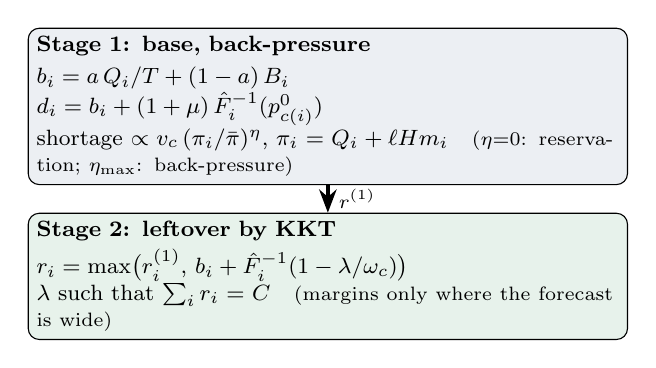
\begin{tikzpicture}[font=\footnotesize,>=Stealth,
   s/.style={draw,rounded corners,align=left,text width=7.4cm,inner sep=3pt}]
  \node[s,fill=iitblue!8] (st1) {\textbf{Stage 1: base, back-pressure}\\[2pt]
    $b_i = a\,Q_i/T + (1-a)\,B_i$\\
    $d_i = b_i + (1+\mu)\,\hat F_i^{-1}(p^0_{c(i)})$\\
    shortage $\propto v_{c}\,(\pi_i/\bar\pi)^{\eta}$, $\pi_i = Q_i + \ell H m_i$\quad{\scriptsize($\eta{=}0$: reservation;\ $\eta_{\max}$: back-pressure)}};
  \node[s,fill=good!10,below=0.35cm of st1] (st2) {\textbf{Stage 2: leftover by KKT}\\[2pt]
    $r_i = \max\!\big(r_i^{(1)},\, b_i + \hat F_i^{-1}(1 - \lambda/\omega_{c})\big)$\\
    $\lambda$ such that $\sum_i r_i = C$\quad{\scriptsize(margins only where the forecast is wide)}};
  \draw[->,very thick] (st1) -- node[right,font=\scriptsize]{$r^{(1)}$} (st2);
\end{tikzpicture}\\[3pt]
\begin{tcolorbox}[enhanced,colback=gold!12,colframe=gold!80!black,boxrule=0.5pt,arc=2pt,left=4pt,right=4pt]
\footnotesize\textbf{Contains both strongest baselines exactly} (unit-tested): predictive MaxWeight ($a{=}1$, $p^0{=}0.5$, $\eta{=}\eta_{\max}$) and the CEM policy ($a{=}0$, $\eta{=}0$).\\
8 parameters learned by CEM on \emph{training} seeds, started from both baselines' optima; baselines re-tuned with the \textbf{same search} for equal effort.
\end{tcolorbox}
\end{column}
\end{columns}
\end{frame}

% ---------------------------------------------------------------------
\begin{frame}{B3 (final) \textbullet\ BPN beats the best baseline in 10/10 scenarios}
\begin{columns}[c]
\begin{column}{0.5\textwidth}
\centering
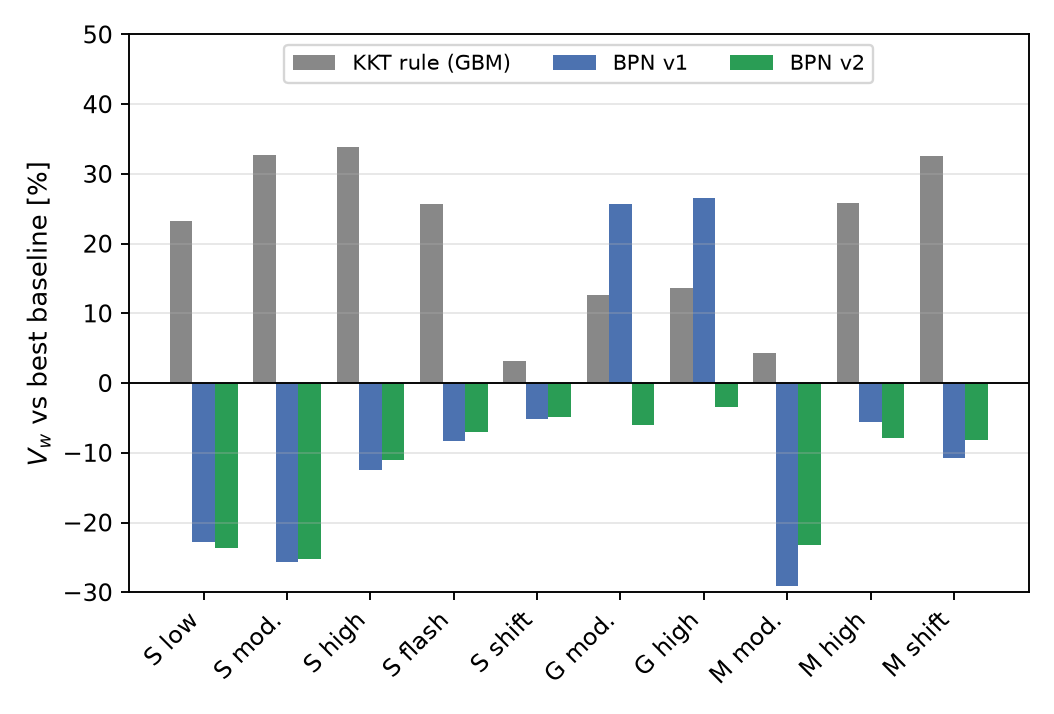
\includegraphics[width=\linewidth]{fig_bpn_vs_best.png}\\
{\scriptsize relative $V_w$ vs the best baseline per scenario: B1 KKT (grey), BPN v1 (blue), BPN v2 (green)}
\end{column}
\begin{column}{0.48\textwidth}
\scriptsize
\setlength{\tabcolsep}{3pt}
\begin{tabular}{lcc|lcc}
\toprule
Scen. & $\Delta V_w$ & seeds & Scen. & $\Delta V_w$ & seeds \\
\midrule
S low & \gd{$-23.7\%$} & 15 & G mod. & \gd{$-5.9\%$} & 20 \\
S mod. & \gd{$-25.3\%$} & 20 & G high & \gd{$-3.4\%$} & 19 \\
S high & \gd{$-11.0\%$} & 20 & M mod. & \gd{$-23.3\%$} & 20 \\
S flash & \gd{$-7.0\%$} & 20 & M high & \gd{$-7.9\%$} & 20 \\
S shift & \gd{$-4.8\%$} & 20 & M shift & \gd{$-8.2\%$} & 20 \\
\bottomrule
\end{tabular}\\[3pt]
{\scriptsize paired over 20 test seeds, Holm--Wilcoxon, all $p \le 0.024$; best baseline = better of predictive MaxWeight and CEM, each in its best tuning with the same search budget}
\vspace{0.5em}
\begin{takeaway}
\footnotesize BPN wins \textbf{every} scenario by 3--25\,\%, on synthetic, 3GPP and Markov traffic, including held-out shifts.
\end{takeaway}
\end{column}
\end{columns}
\end{frame}

% ---------------------------------------------------------------------
\begin{frame}{B3 (final) \textbullet\ What the BPN policy learned}
\begin{columns}[T]
\begin{column}{0.48\textwidth}
\footnotesize
\textbf{\small Learned parameters} (BPN v2)\\[3pt]
\begin{tabular}{lccc}
\toprule
Family & $\eta$ & $a$ & $(p^0_{\rm LL}, p^0_{\rm eMBB})$ \\
\midrule
S (bursty) & 6: back-pressure & 0.98 & (0.41, 0.45) \\
G (3GPP) & 0: reservation & 0.31 & (0.94, 0.73) \\
M (Markov) & 0: reservation & 0.34 & (0.84, 0.31) \\
\bottomrule
\end{tabular}
\end{column}
\begin{column}{0.5\textwidth}
\begin{itemize}\footnotesize
  \item The search \textbf{recovers the regime map}: back-pressure for short bursts, reservation for long ones.
  \item With Bayesian LCQT: \textbf{5.05\,\%} at S high, within 6--10\,\% of the oracle-informed rule.
  \item 2.2--3.5\,ms per decision, well inside the 10\,ms interval.
\end{itemize}
\end{column}
\end{columns}
\vspace{0.2em}
\centering
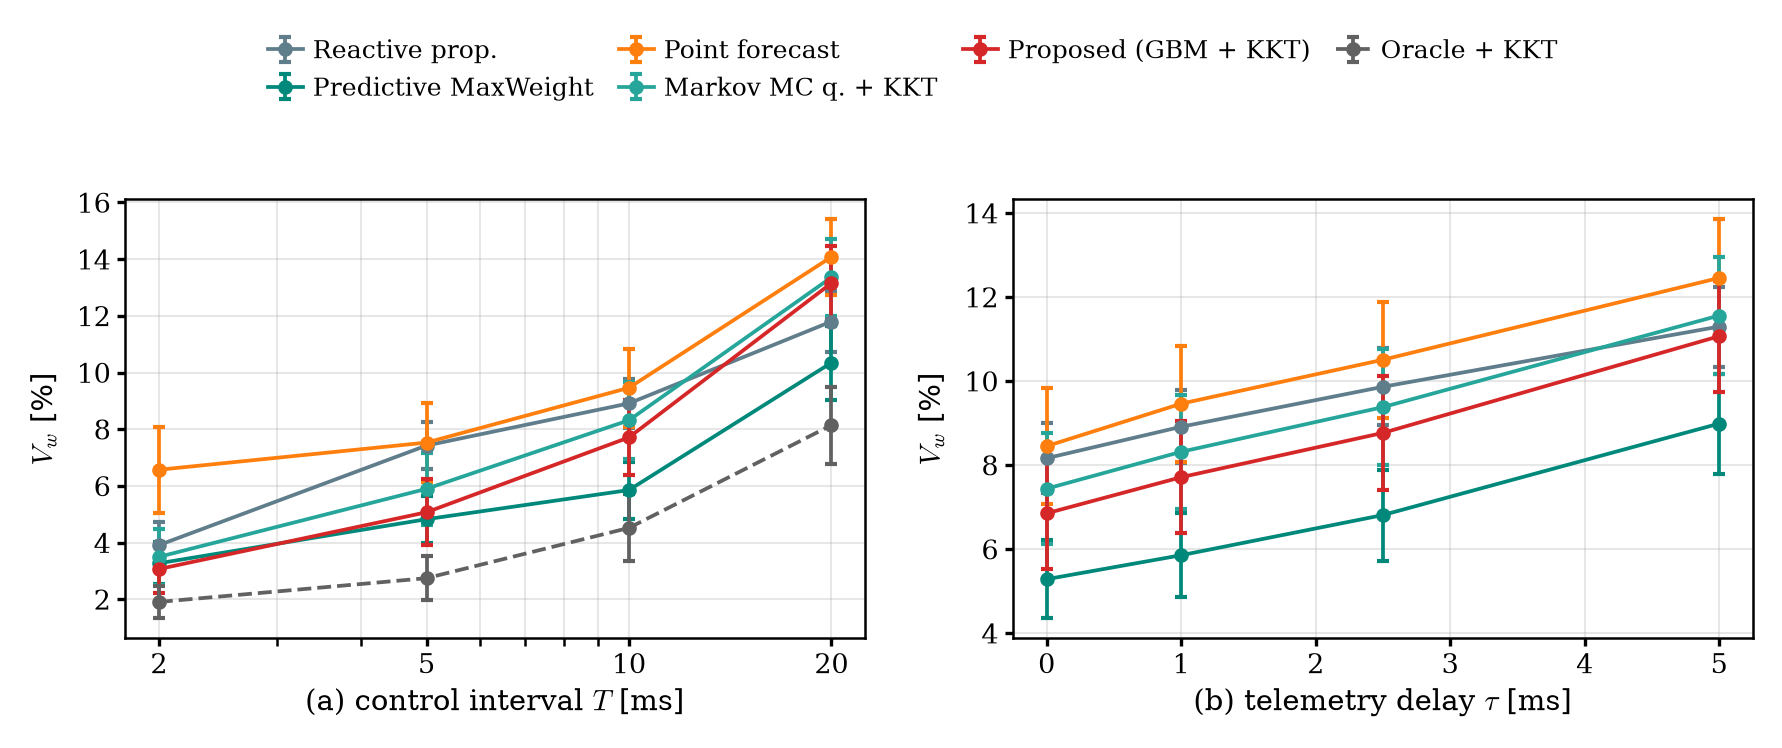
\includegraphics[width=0.6\linewidth]{paper_fig_regime.png}\\
{\scriptsize S high, $V_w$ vs interval $T$ and delay $\tau$: back-pressure (pred.\ MaxWeight) wins at 10--20\,ms intervals, reservation (KKT) at short ones.}
\end{frame}

% =====================================================================
\section{Wrap-up}
% =====================================================================

\begin{frame}{Implementation and reproducibility}
\begin{columns}[T]
\begin{column}{0.53\textwidth}
\scriptsize
\renewcommand{\arraystretch}{1.15}
\setlength{\tabcolsep}{3pt}
\begin{tabular}{>{\ttfamily}p{2.75cm} p{4.4cm}}
\toprule
\normalfont Module & Content \\
\midrule
matinv\_bench/ & inversion benchmark, InverseNets \\
cmatinv/, exp.\_v2/ & complex inversion, RMT-WS, 38.901 \\
kernels/ (\texttt{libcmat}) & fused C/AVX-512/OpenMP library \\
fhlm/ & simulator, families S/G/M, 19+ ctrl. \\
fhlm/transformer.py & B2: LCQT, mixture, diff.\ KKT \\
fhlm/hybrid.py & B3: BPN + equal-budget CEM \\
tests/ & 46 unit tests \\
results/ & all CSVs, logs, figures \\
\bottomrule
\end{tabular}
\end{column}
\begin{column}{0.45\textwidth}
\footnotesize
\begin{itemize}
  \item \textbf{Slot-accurate simulator}: stale observations, held budgets, FIFO deadline drops, every metric logged.
  \item \textbf{Tests} check: capacity in every slot, no future leakage, $\rstar$ tightness, bound validity, KKT-layer gradients, BPN containment.
  \item Every number in the papers is a \textbf{macro generated from the CSVs}.
  \item Decision time (Python): KKT + GBM 3.5\,ms, BPN 2.2--3.5\,ms, inside the 10\,ms interval.
\end{itemize}
\end{column}
\end{columns}
\vspace{0.3em}
\begin{takeaway}
\faIcon[regular]{file-alt}\ \ B1 paper submitted to \textbf{NCC 2027}; 11-page extended manuscript with theory, three families and 19 controllers; \texttt{libcmat} being prepared as an open-source library and publication.
\end{takeaway}
\end{frame}

% ---------------------------------------------------------------------
\begin{frame}{Conclusions}
\begin{columns}[T]
\begin{column}{0.49\textwidth}
\begin{block}{\faIcon{compress-arrows-alt}\ \ Part A: lighter fronthaul, real-time DU}
\footnotesize
\begin{itemize}
  \item CSEE / RAS-BFP: \textbf{6.4--8.1$\times$} vs 16-bit IQ at $\approx-20$\,dB (BFP 2$\times$), with error bounds, \textbf{3--6$\times$ faster} than SVD.
  \item RMT-WS: \textbf{6 GEMMs} instead of $>10$; certified warm start at every speed; closed-form Doppler law.
  \item \texttt{libcmat}: whole precoder \textbf{0.226\,ms} (14$\times$ numpy + LAPACK), inverse 14$\times$ LAPACK, inside the slot.
  \item RU-side precoding: \textbf{$-72\,\%$} fronthaul at 99.7\,\% sum-rate.
\end{itemize}
\end{block}
\end{column}
\begin{column}{0.49\textwidth}
\begin{block}{\faNetworkWired\ \ Part B: smarter sharing}
\footnotesize
\begin{itemize}
  \item $\rstar$ turns deadlines into a demand target; the KKT rule splits at equal weighted risk.
  \item B1: best of 12 controllers on 2 families, \textbf{$-11$ to $-43\,\%$} vs point forecast.
  \item B2: Bayesian LCQT, uncertainty-aware and explainable, best calibration, improves B1 on every seed.
  \item \textbf{B3 (final)}: BPN beats the strongest baselines in \textbf{10/10} scenarios of 3 families, \textbf{3--25\,\%}.
\end{itemize}
\end{block}
\end{column}
\end{columns}
\vspace{0.4em}
\begin{tcolorbox}[enhanced,colback=good!8,colframe=good,boxrule=0.6pt,arc=3pt,halign=center]
\small\textbf{One system:} Part A lowers the load on the link; Part B serves what remains with the right capacity at the right time. Compression sets the regime, allocation decides the loss inside it.
\end{tcolorbox}
\end{frame}

% ---------------------------------------------------------------------
\begin{frame}{Scope and future work}
\begin{columns}[T]
\begin{column}{0.49\textwidth}
\begin{block}{\faIcon{bullseye}\ \ Scope of the results}
\footnotesize
\begin{itemize}
  \item CSEE and RAS-BFP target \textbf{channel-carrying IQ} (reference signals, RU-side precoding weights); data-symbol IQ stays on standard BFP.
  \item \texttt{libcmat} is tuned for the O-DU regime: many small complex Hermitian systems ($K \le 32$) per slot on AVX-512 CPUs.
  \item The KKT rule is designed for differentiated priorities and decision intervals up to a few deadlines; BPN covers the remaining regimes.
  \item BPN parameters are learned per traffic family at $T{=}10$\,ms, $\tau{=}1$\,ms, the near-RT RIC operating point.
\end{itemize}
\end{block}
\end{column}
\begin{column}{0.49\textwidth}
\begin{exampleblock}{Next steps}
\footnotesize
\begin{itemize}
  \item \faBook\ \ Release \texttt{libcmat} as an open-source library and publish it.
  \item \faMicrochip\ \ GPU / NPU / tensor-core port of the Newton--Schulz kernel and certificate.
  \item \faRobot\ \ BPN as the structured policy of a PPO \textbf{xApp} in the near-RT RIC, with the KKT rule as safe fallback.
  \item \faBolt\ \ Compiled (C++/ONNX) Bayesian forecaster for the 10\,ms decision loop.
  \item \faSlidersH\ \ Joint per-cell knob: BFP width \emph{and} capacity share every interval.
  \item \faIcon{exchange-alt}\ \ Cross-family transfer and online adaptation over A1.
\end{itemize}
\end{exampleblock}
\end{column}
\end{columns}
\end{frame}

% ---------------------------------------------------------------------
{
\setbeamercolor{background canvas}{bg=iitblue}
\begin{frame}[plain,noframenumbering]
\centering
\vspace{1.2cm}
{\color{white}\fontsize{34}{40}\selectfont\bfseries Thank you}\\[0.4cm]
{\color{gold}\rule{3cm}{1.5pt}}\\[0.5cm]
{\color{white}\Large Questions?}\\[1.3cm]
{\color{white}\small Harshvardhan Choudhary \quad\textbullet\quad Mayank Yadav}\\[3pt]
{\color{white!80!iitblue}\footnotesize Guide: Dr.~Sumit Gautam \,\textbullet\, Department of Electrical Engineering \,\textbullet\, IIT Indore}
\end{frame}
}

% =====================================================================
\appendix
% =====================================================================

\begin{frame}[noframenumbering]{Backup: paired per-seed reductions of the KKT rule (Family S)}
\centering
\scriptsize
\begin{tabular}{lccccc}
\toprule
Proposed vs. & low & moderate & high & flash crowds & shift \\
\midrule
Reactive proportional & $-81\,\%$ 20/20** & $-48\,\%$ 20/20** & $-13\,\%$ 20/20** & \hl{$-4\,\%$ 16/20*} & $-14\,\%$ 20/20** \\
MaxWeight & $-83\,\%$ 20/20** & $-56\,\%$ 20/20** & $-31\,\%$ 20/20** & $-23\,\%$ 20/20** & $-18\,\%$ 20/20** \\
Deadline-aware reactive & $-70\,\%$ 20/20** & $-49\,\%$ 20/20** & $-27\,\%$ 20/20** & $-19\,\%$ 20/20** & $-20\,\%$ 20/20** \\
Point forecast & $-43\,\%$ 20/20** & $-33\,\%$ 20/20** & $-18\,\%$ 20/20** & $-12\,\%$ 20/20** & $-11\,\%$ 20/20** \\
Fixed global quantile & $-54\,\%$ 20/20** & $-50\,\%$ 20/20** & $-32\,\%$ 20/20** & $-22\,\%$ 20/20** & $-22\,\%$ 20/20** \\
Window quantiles (no ML) & $-37\,\%$ 20/20** & $-16\,\%$ 20/20** & $-8\,\%$ 20/20** & $-7\,\%$ 20/20** & $-2\,\%$ 16/20** \\
\bottomrule
\end{tabular}\\[3pt]
{\tiny mean relative change of $V_w$, seeds won out of 20; ** Holm--Wilcoxon $p<0.01$, * $p<0.05$}\\[6pt]
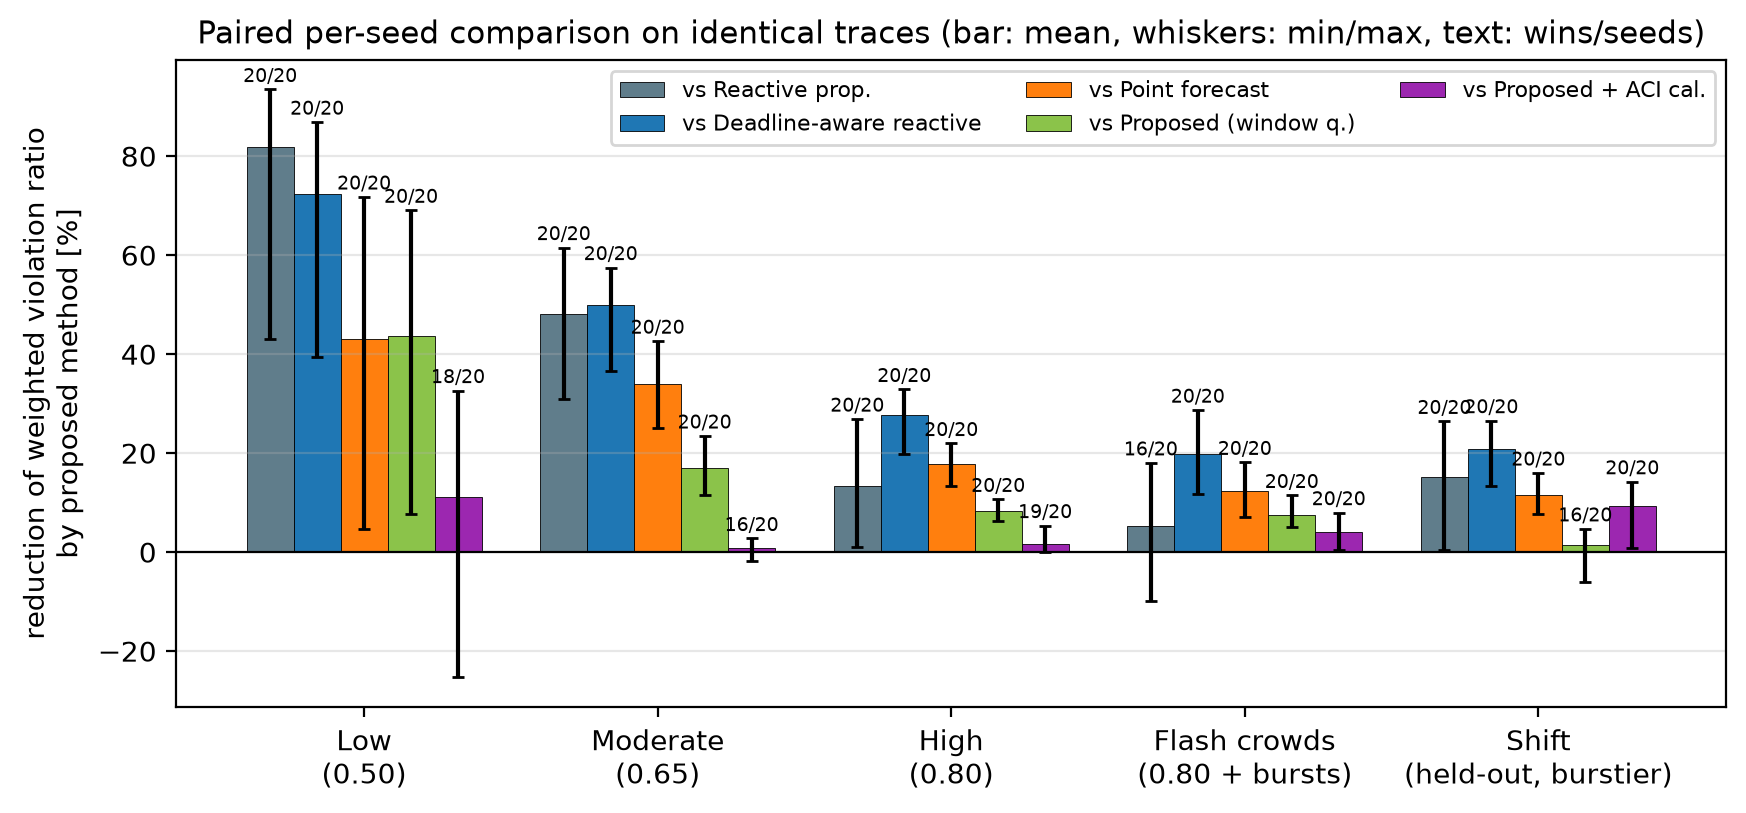
\includegraphics[width=0.62\linewidth]{fig8_paired_reduction.png}
\end{frame}

\begin{frame}[noframenumbering]{Backup: BPN on Families G and M, and all 19 controllers}
\begin{columns}[c]
\begin{column}{0.52\textwidth}
\scriptsize
\setlength{\tabcolsep}{3pt}
\begin{tabular}{lccccc}
\toprule
$V_w$ [\%], GBM & G mod. & G high & M mod. & M high & M shift \\
\midrule
KKT rule (B1) & 5.08 & 8.01 & 0.92 & 4.94 & 5.52 \\
Pred.\ MaxW.\ (CEM) & 6.75 & 10.02 & 1.61 & 4.82 & 4.82 \\
CEM (re-searched) & 4.51 & 7.05 & 0.94 & 3.94 & 4.22 \\
BPN v1 & 5.67 & 8.92 & \textbf{0.63} & 3.71 & \textbf{3.72} \\
\ours \textbf{BPN v2} & \textbf{4.24} & \textbf{6.81} & 0.68 & \textbf{3.62} & 3.82 \\
\gray{Oracle + KKT} & \gray{3.47} & \gray{6.06} & \gray{0.03} & \gray{1.84} & \gray{2.31} \\
\bottomrule
\end{tabular}\\[4pt]
\end{column}
\begin{column}{0.44\textwidth}
\footnotesize BPN v1 (stage 1 always strict back-pressure) cannot represent reservation and loses on G; v2's exponent $\eta$ contains it and generalises.
\end{column}
\end{columns}
\vspace{0.3em}
\centering
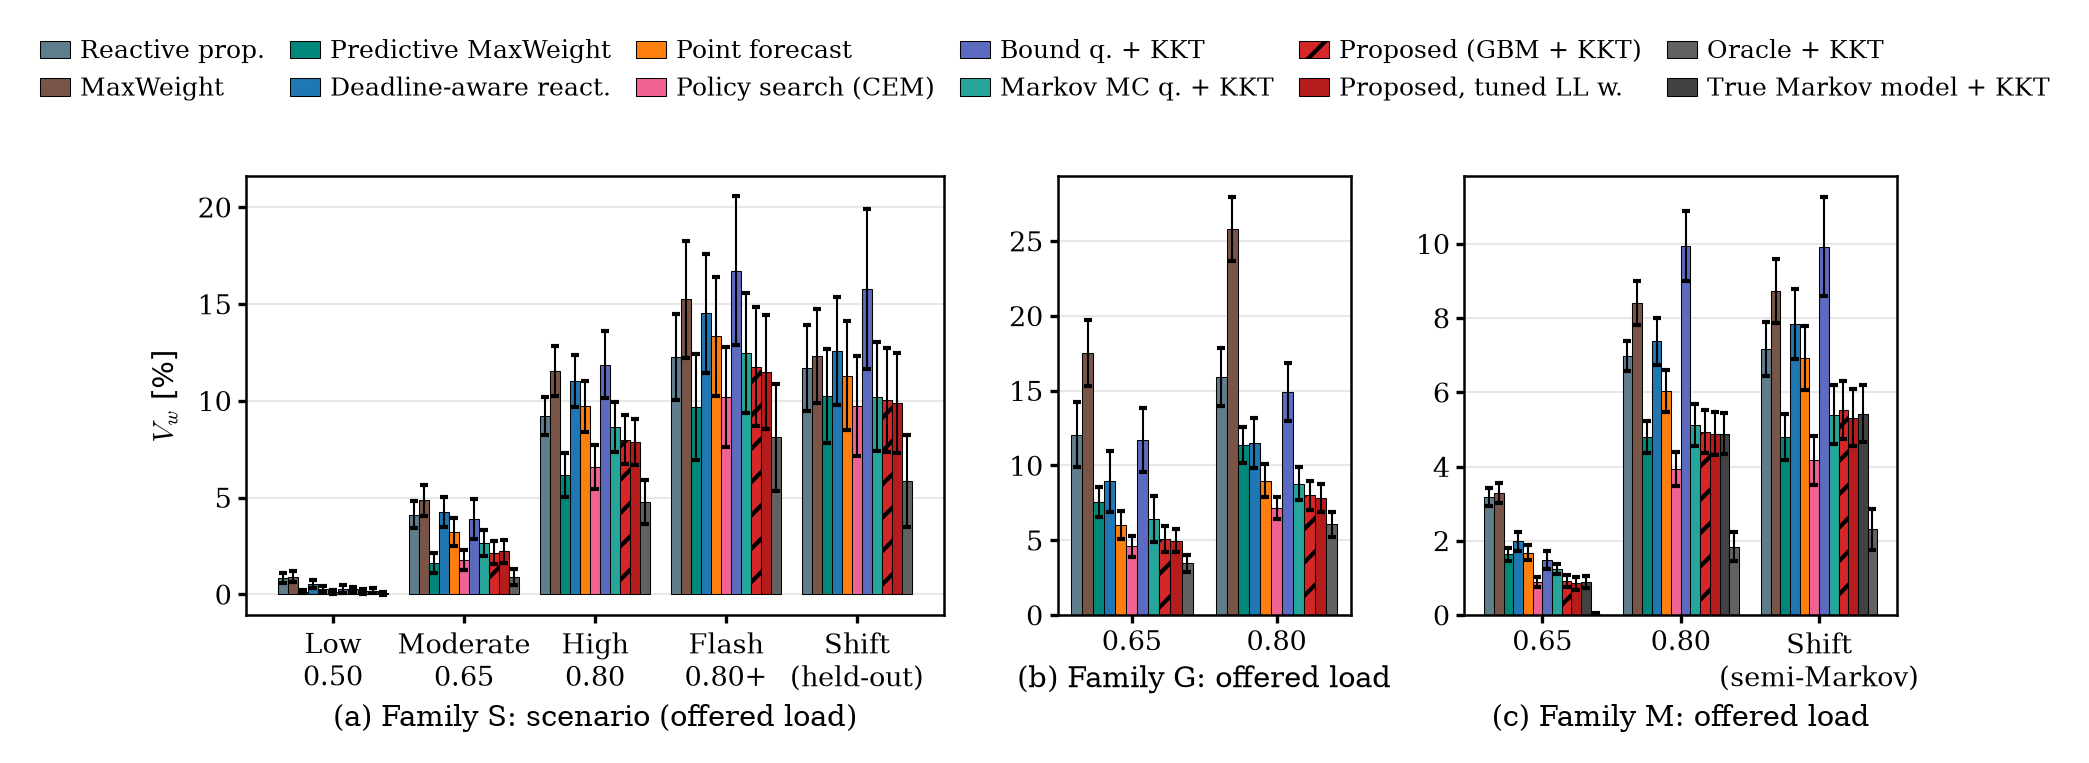
\includegraphics[width=0.85\linewidth]{paper_fig_overview_ext.png}
\end{frame}

\begin{frame}[noframenumbering]{Backup: likely questions}
\small
\begin{description}[Why GBM, not LSTM?]
  \item[Leakage?] Train seeds 1000--1015, val 2000--2003, test 3000--3019; forecasters frozen before test; features use past slots only (tested).
  \item[Why GBM first?] Six quantile models train in 12\,s, calibrated, CPU-only; the ablation shows the rule carries most of the gain. B2 then replaces it with LCQT.
  \item[Why beat LAPACK?] LAPACK is tuned for one large matrix; the O-DU solves 273 small Hermitian systems per slot. \texttt{libcmat} fuses Gram, inverse and weights per PRB in L1, vectorises re/im planes and threads across PRBs.
  \item[Is it optimal?] KKT is the global optimum of the one-interval surrogate only; no closed-loop optimality claim.
  \item[Why not deep RL?] CEM on a structured policy class is a small, reliable analogue of an RL xApp; a PPO xApp with BPN as policy class is future work.
  \item[Compressing data IQ?] No: QAM data destroys low rank and delay sparsity; data IQ stays on BFP.
\end{description}
\end{frame}

\begin{frame}[noframenumbering]{Backup: key references}
\scriptsize
\begin{itemize}
  \item O-RAN WG4, \emph{Control, User and Synchronization Plane Specification} (split 7-2x, BFP). \quad 3GPP TR 38.801, TR 38.901, TS 38.214, TR 36.814, TR 38.838.
  \item L.\,M.\,P.\ Larsen, A.\ Checko, H.\,L.\ Christiansen, ``A survey of the functional splits proposed for 5G mobile crosshaul networks,'' \emph{IEEE COMST}, 2019.
  \item S.\ Lag\'en et al., ``Fronthaul compression control for shared fronthaul access networks,'' \emph{IEEE Commun.\ Mag.}, 2022.
  \item N.\ Halko, P.\,G.\ Martinsson, J.\,A.\ Tropp, ``Finding structure with randomness,'' \emph{SIAM Review}, 2011.
  \item M.\ Wu et al.\ (2013), D.\ Prabhu et al.\ (2013): Neumann-series detection; H.\ Shao et al.\ (2016): Newton--Neumann.
  \item V.\,A.\ Marchenko, L.\,A.\ Pastur, eigenvalue distribution of random matrices, 1967.
  \item D.\ Bega et al., DeepCog (2019) and AZTEC (2020): forecast-driven capacity allocation.
  \item G.\ Hadley, T.\,M.\ Whitin, \emph{Analysis of Inventory Systems} (multi-item newsvendor), 1963. \quad J.-Y.\ Le Boudec, P.\ Thiran, \emph{Network Calculus}, 2001.
  \item L.\ Tassiulas, A.\ Ephremides, MaxWeight, 1992; L.\ Huang et al., predictive back-pressure, 2016; R.\,Y.\ Rubinstein, cross-entropy method, 1999.
  \item D.\ Anick, D.\ Mitra, M.\,M.\ Sondhi, Markov fluid sources, \emph{BSTJ}, 1982; F.\,P.\ Kelly, effective bandwidths, 1996.
  \item Y.\ Nie et al., PatchTST, ICLR 2023; Y.\ Liu et al., iTransformer, ICLR 2024; B.\ Lim et al., TFT, \emph{IJF} 2021.
  \item Y.\ Gal, Z.\ Ghahramani, MC dropout, 2016; B.\ Lakshminarayanan et al., deep ensembles, 2017; P.\ Donti et al., task-based learning, 2017.
\end{itemize}
\end{frame}

\end{document}
